\documentclass[11pt]{article}

% ══════════════════════════════════════════════════════════════════════════════
%  PACKAGES
% ══════════════════════════════════════════════════════════════════════════════
\usepackage[T1]{fontenc}
\usepackage[utf8]{inputenc}
\usepackage{amsmath,amssymb,amsfonts,amsthm}
\usepackage{graphicx}
\graphicspath{{figures/}}
\usepackage{bm}
\usepackage{siunitx}
\usepackage{geometry}
\usepackage[colorlinks=true,linkcolor=black,citecolor=blue,urlcolor=blue]{hyperref}
\usepackage[noabbrev,nameinlink]{cleveref}
\usepackage{xcolor}
\usepackage{booktabs}
\usepackage{enumitem}
\usepackage{float}

\geometry{margin=1in}

% ══════════════════════════════════════════════════════════════════════════════
%  TITLE
% ══════════════════════════════════════════════════════════════════════════════
\title{A Theoretical Framework for Parameter Investigation\\
       of Self-Starting Siphons\\[0.75em]
       \rule{0.7\textwidth}{0.4pt}\\[0.75em]
       \large IYPT 2026 --- Problem \#1}
\author{Stelios Raptopoulos}
\date{December 2024}

\begin{document}
\maketitle

% ══════════════════════════════════════════════════════════════════════════════
%  ABSTRACT
% ══════════════════════════════════════════════════════════════════════════════
\begin{abstract}
A self-starting siphon primes spontaneously when partially immersed, without external suction. This paper develops a one-dimensional slug-flow model through layered analysis, progressively adding physical effects to identify how parameters control priming success and filling time. The theoretical framework is validated against a laboratory experiment using a siphon constructed from drinking straws; the experimental geometry and measurements serve as the worked example throughout.

The analysis begins with the frictionless case, where geometry alone determines the outcome. The driving force $F = \rho g A [h_c - h(L)]$ depends only on the elevation difference between the container surface and the advancing front. This yields an energy integral $I(L)$ computable in closed form for piecewise-linear geometries. The priming criterion $I(S_W) > 0$ provides a geometric screening tool.

Container drawdown is added next, introducing the area ratio $A/A_0$ as the controlling parameter. The modified integral $I_{\text{dd}}(L)$ remains analytical. Friction is then incorporated through a constant-friction approximation, yielding a third integral $I_f(L)$ that reveals how dissipation discounts early-stored energy. Comparing these three integrals on a single graph shows how each effect reduces the available kinetic energy.

The full dynamics require numerical integration due to velocity-dependent friction, but the analytical integrals bracket the solution and provide physical insight. The draining phase following successful priming is treated in full. A systematic derivation from Navier-Stokes makes every assumption explicit, bridging to validity limits: cavitation, capillarity, entrance effects, and unsteady friction are quantified through dimensionless parameters and visualised in regime diagrams.

The framework enables systematic parameter investigation by revealing how geometry, pipe properties, and system size each affect the siphoning process.
\end{abstract}

\tableofcontents
\newpage

% ══════════════════════════════════════════════════════════════════════════════
%  SECTION 1: INTRODUCTION
% ══════════════════════════════════════════════════════════════════════════════
\section{Introduction}
\label{sec:intro}

The International Young Physicists' Tournament (IYPT) 2026 Problem~\#1 states:
\begin{quote}
\emph{``A self-starting siphon can be made using a piece of rigid tubing bent into a specific shape. When the siphon is partially immersed in water, it begins siphoning water without the need for initial suction. Investigate how the relevant parameters, such as the geometry, affect the siphoning process.''}
\end{quote}

A conventional siphon requires priming: the tube must be filled with water before operation. A self-starting siphon eliminates this step through geometry alone. When partially submerged, water enters the pipe, gains momentum descending an internal drop, and uses that momentum to climb over a crest above the waterline. Once primed, ordinary siphon action drains the container.

The question is: what makes this work, and how do the parameters control it?

\subsection{Approach}

This paper develops a theoretical framework through layered analysis:

\begin{enumerate}[nosep,leftmargin=2em]
  \item \textbf{Frictionless model} (\cref{sec:frictionless}): Geometry alone determines priming. The energy integral $I(L)$ provides a closed-form criterion.
  \item \textbf{Adding drawdown} (\cref{sec:drawdown}): The area ratio $A/A_0$ controls how the container level drops, modifying the driving force.
  \item \textbf{Adding friction} (\cref{sec:friction}): Pipe roughness $\varepsilon/D$ and bend losses $K$ dissipate energy, captured analytically through $I_f(L)$.
  \item \textbf{Model comparison} (\cref{sec:comparison}): The three integrals are compared on the same graph to visualise each effect.
  \item \textbf{Full dynamics} (\cref{sec:dynamics}): Velocity-dependent friction requires numerical integration. Draining is treated in full.
  \item \textbf{Foundations} (\cref{sec:navier-stokes}): Derivation from Navier-Stokes makes assumptions explicit.
  \item \textbf{Validity limits} (\cref{sec:validity}): Dimensionless parameters quantify when the model breaks down.
\end{enumerate}

Each layer introduces one key parameter while preserving analytical tractability as long as possible. A laboratory experiment provides the worked example: the experimental geometry and velocity measurements are used throughout to test each successive model. The goal is not optimal design but understanding: how does each parameter affect the siphoning process?

% ══════════════════════════════════════════════════════════════════════════════
%  SECTION 2: PHYSICAL SETUP
% ══════════════════════════════════════════════════════════════════════════════
\section{The Physical Setup}
\label{sec:setup}

\subsection{Coordinate system}

We work in a vertical plane with coordinates $(x, h)$: $x$ horizontal (rightward positive), $h$ vertical (upward positive). The datum $h = 0$ is at the container base.

\subsection{The five-node geometry}

The pipe centreline connects five nodes by straight segments:
\[
  A = (x_0, h_0), \quad B = (x_1, h_1), \quad C = (x_2, h_2), \quad D = (x_3, h_3), \quad E = (x_4, h_4).
\]

Each node has a physical role:
\begin{center}
\renewcommand{\arraystretch}{1.2}
\begin{tabular}{cl}
\toprule
Node & Role \\
\midrule
$A$ & Inlet, near container bottom \\
$B$ & First crest, below initial water level \\
$C$ & Low point of internal drop, where velocity peaks \\
$D$ & Main crest, \emph{above} the initial water level \\
$E$ & Outlet, at or below container bottom \\
\bottomrule
\end{tabular}
\end{center}

The defining constraint for self-starting is $h_1 < h_c^{(0)} < h_3$: the first crest lies below the waterline, the main crest above it.

\subsection{The worked example: experimental parameters}
\label{sec:worked-example}

The theoretical framework is developed around a specific siphon geometry that was constructed and tested in the laboratory. All numerical examples throughout this paper use the parameters from this experiment, allowing direct comparison between theoretical predictions and measured behaviour. \Cref{tab:parameters} defines every parameter; subsequent sections reference this table rather than re-introducing values.

\begin{table}[H]
\centering
\caption{Complete parameter set for the worked example (experimental setup).}
\label{tab:parameters}
\renewcommand{\arraystretch}{1.2}
\small
\begin{tabular}{llll}
\toprule
\multicolumn{4}{l}{\textbf{Geometric parameters}} \\
\midrule
Node & $x$ (cm) & $h$ (cm) & Description \\
\midrule
$A$ & 0.0 & 1.0 & Inlet \\
$B$ & 7.5 & 11.0 & First crest (1.5\,cm below waterline) \\
$C$ & 13.5 & 5.0 & Low point \\
$D$ & 21.4 & 13.0 & Main crest (0.5\,cm above waterline) \\
$E$ & 30.3 & $-1.7$ & Outlet \\
\midrule
\multicolumn{4}{l}{Initial water level: $h_c^{(0)} = 12.5$\,cm} \\
\midrule
\multicolumn{4}{l}{\textbf{Segment properties}} \\
\midrule
Segment & Length $L_i$ (cm) & Slope $s_i$ & Role \\
\midrule
$A \to B$ & 12.50 & $+0.800$ & Initial rise \\
$B \to C$ & 8.49 & $-0.707$ & Momentum-building drop \\
$C \to D$ & 11.24 & $+0.712$ & Climb to crest \\
$D \to E$ & 17.18 & $-0.855$ & Descent to outlet \\
\midrule
\multicolumn{4}{l}{Total pipe length: $L_{\max} = 49.41$\,cm} \\
\midrule
\multicolumn{4}{l}{\textbf{Cumulative arclengths}} \\
\midrule
Symbol & Value (cm) & \multicolumn{2}{l}{Location} \\
\midrule
$S_0$ & 0 & \multicolumn{2}{l}{Node $A$ (inlet)} \\
$S_1$ & 12.50 & \multicolumn{2}{l}{Node $B$ (first crest)} \\
$S_2$ & 20.99 & \multicolumn{2}{l}{Node $C$ (low point)} \\
$S_{W'}$ & 31.53 & \multicolumn{2}{l}{Point $W'$ (ascending waterline crossing)} \\
$S_3$ & 32.23 & \multicolumn{2}{l}{Node $D$ (main crest)} \\
$S_W$ & 32.81 & \multicolumn{2}{l}{Point $W$ (last waterline crossing)} \\
$S_4$ & 49.41 & \multicolumn{2}{l}{Node $E$ (outlet)} \\
\midrule
\multicolumn{4}{l}{\textbf{Pipe parameters}} \\
\midrule
Parameter & Value & \multicolumn{2}{l}{Description} \\
\midrule
$D$ & 5\,mm & \multicolumn{2}{l}{Inner diameter} \\
$A = \pi D^2/4$ & $0.196\,\text{cm}^2$ & \multicolumn{2}{l}{Cross-sectional area} \\
$\varepsilon/D$ & $3.5\times 10^{-4}$ & \multicolumn{2}{l}{Relative roughness (estimate; weakly identifiable at low Re)} \\
$\sum K$ & 14.4 & \multicolumn{2}{l}{Effective minor loss coefficient (fit to $v(L)$)} \\
\midrule
\multicolumn{4}{l}{\textbf{System parameters}} \\
\midrule
$A_0$ & $340\,\text{cm}^2$ & \multicolumn{2}{l}{Container cross-sectional area} \\
$A/A_0$ & $5.77\times 10^{-4}$ & \multicolumn{2}{l}{Area ratio} \\
$\rho$ & $998\,\text{kg/m}^3$ & \multicolumn{2}{l}{Water density at $20^\circ$C} \\
$\mu$ & $1.0 \times 10^{-3}\,\text{Pa}\cdot\text{s}$ & \multicolumn{2}{l}{Dynamic viscosity} \\
$\nu$ & $1.0 \times 10^{-6}\,\text{m}^2/\text{s}$ & \multicolumn{2}{l}{Kinematic viscosity} \\
$\gamma$ & $0.073\,\text{N/m}$ & \multicolumn{2}{l}{Surface tension} \\
$g$ & $9.81\,\text{m/s}^2$ & \multicolumn{2}{l}{Gravitational acceleration} \\
\bottomrule
\end{tabular}
\end{table}

\subsection{Centreline elevation function}

The arclength $L$ measures distance along the pipe from the inlet. On segment $i$ (for $L \in [S_{i-1}, S_i]$), the centreline elevation is linear:
\begin{equation}
  h(L) = c_i + s_i L,
  \label{eq:hL-piecewise}
\end{equation}
where the slope $s_i = (h_i - h_{i-1})/L_i = \sin\theta_i$ and the intercept $c_i = h_{i-1} - s_i S_{i-1}$ ensures continuity.

For the worked example: $c_1 = 1.00$\,cm, $c_2 = 19.84$\,cm, $c_3 = -9.93$\,cm, $c_4 = 40.57$\,cm.

\subsection{Experimental apparatus and data acquisition}

The experiment providing the worked example was conducted as follows. The siphon was constructed from flexible drinking straws arranged in the five-node geometry described above, mounted on simple plastic containers. Video recordings were captured using an iPhone at 4K resolution and 60\,fps. Frame-by-frame motion analysis was performed using free video motion analysis software, available on both mobile and desktop platforms. The water front position was tracked manually in each frame, yielding position-versus-time data from which velocities were computed by numerical differentiation.

The experimental velocity measurements (shown as data points in \cref{fig:comparison,fig:velocity,fig:time}) are compared against model predictions throughout the paper. This low-cost setup demonstrates that the essential physics of self-starting siphons can be investigated without specialised laboratory equipment.

\subsection{Point $W$: the last waterline crossing}

On segment $D \to E$, the front descends from $h_3 = 13$\,cm (above waterline) to $h_4 = -1.7$\,cm (below). Point $W$ is where the front crosses the waterline for the last time:
\[
  h(S_W) = h_c^{(0)} \quad \Rightarrow \quad S_W = \frac{h_c^{(0)} - c_4}{s_4} = \frac{12.5 - 40.57}{-0.855} = 32.81\,\text{cm}.
\]

The front also crosses the waterline on the climb at point $W'$ on segment $C \to D$ at $S_{W'} = 31.53$\,cm. Between $W'$ and $W$, the driving force is negative. Point $W$ is critical: once past it, the driving force is permanently positive and priming is guaranteed.

\subsection{State variables and initial conditions}

The filling process has two state variables:
\begin{itemize}[nosep,leftmargin=2em]
  \item $L(t)$: wetted length (arclength from inlet to front)
  \item $h_c(t)$: container surface elevation
\end{itemize}

The front velocity is $v = \dot{L}$ and the front elevation is $h(L)$.

At $t = 0$, the container has been slowly filled to level $h_c^{(0)}$. Water has entered the pipe and filled segment $A \to B$ hydrostatically, with the front resting at node $B$. A small perturbation tips water over the first crest, initiating dynamic filling.

Initial conditions: $L(0) = S_1 = 12.50$\,cm, $v(0) = 0$.

% --- FIGURE 1: Geometry schematic ---
\begin{figure}[H]
  \centering
  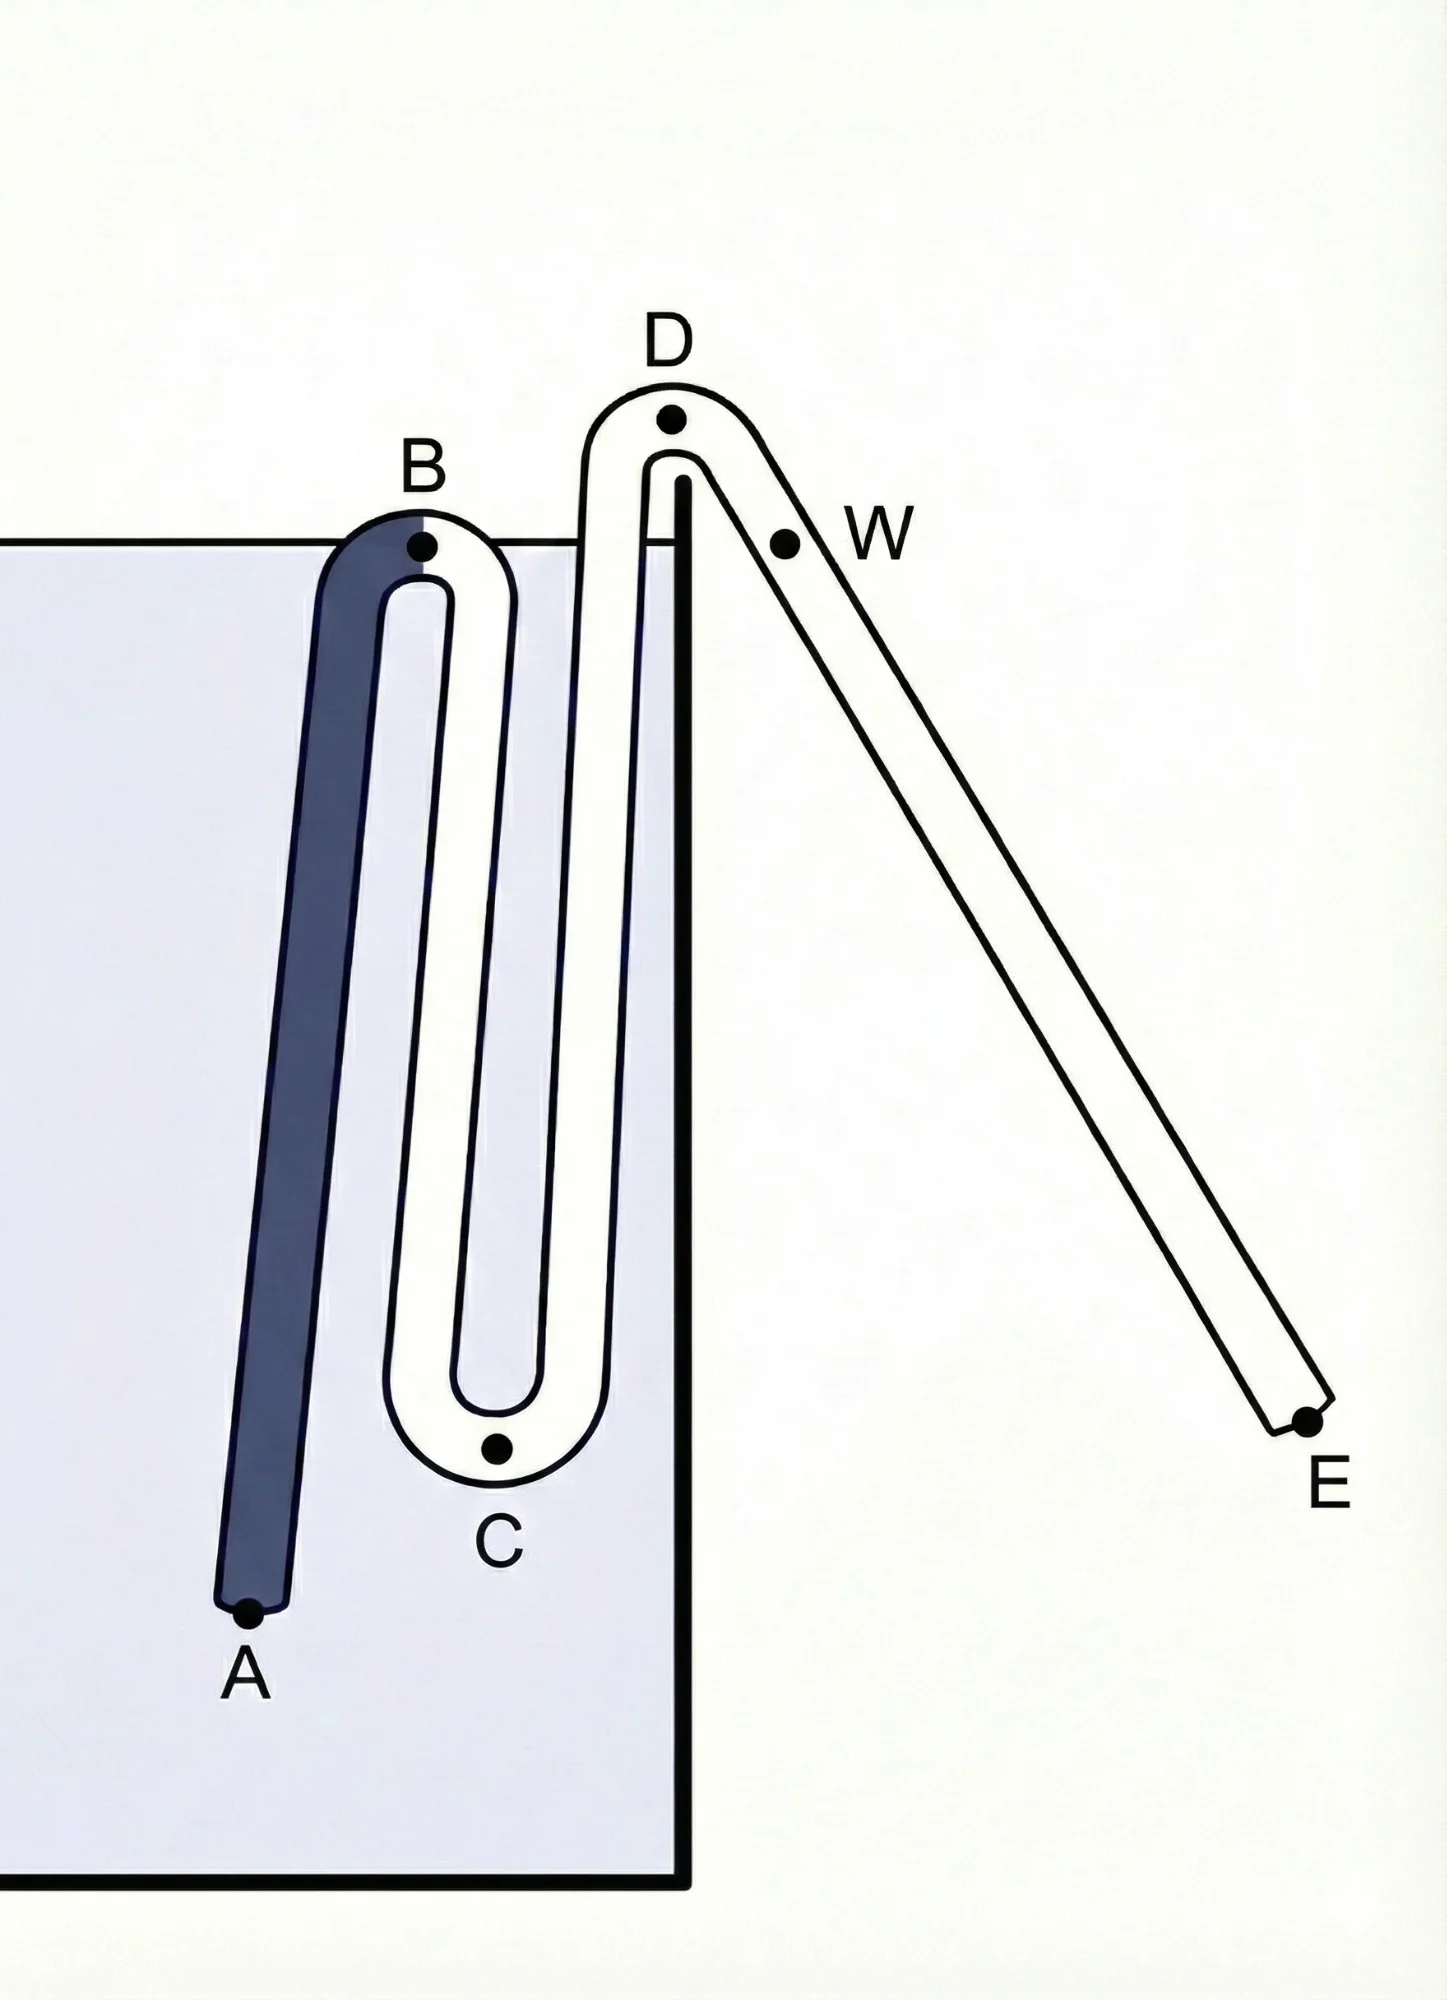
\includegraphics[width=0.6\textwidth]{siphon_schematic.png}
  \caption{Schematic of the self-starting siphon geometry. The container water level $h_c^{(0)}$ lies between the first crest $B$ and main crest $D$. Node $A$ is the inlet; segment $A \to B$ fills hydrostatically. The drop $B \to C$ builds momentum. The climb $C \to D$ passes above the waterline. Point $W$ on segment $D \to E$ marks the last waterline crossing.}
  \label{fig:schematic}
\end{figure}

% --- FIGURE 2: Centreline profile h(L) ---
\begin{figure}[H]
  \centering
  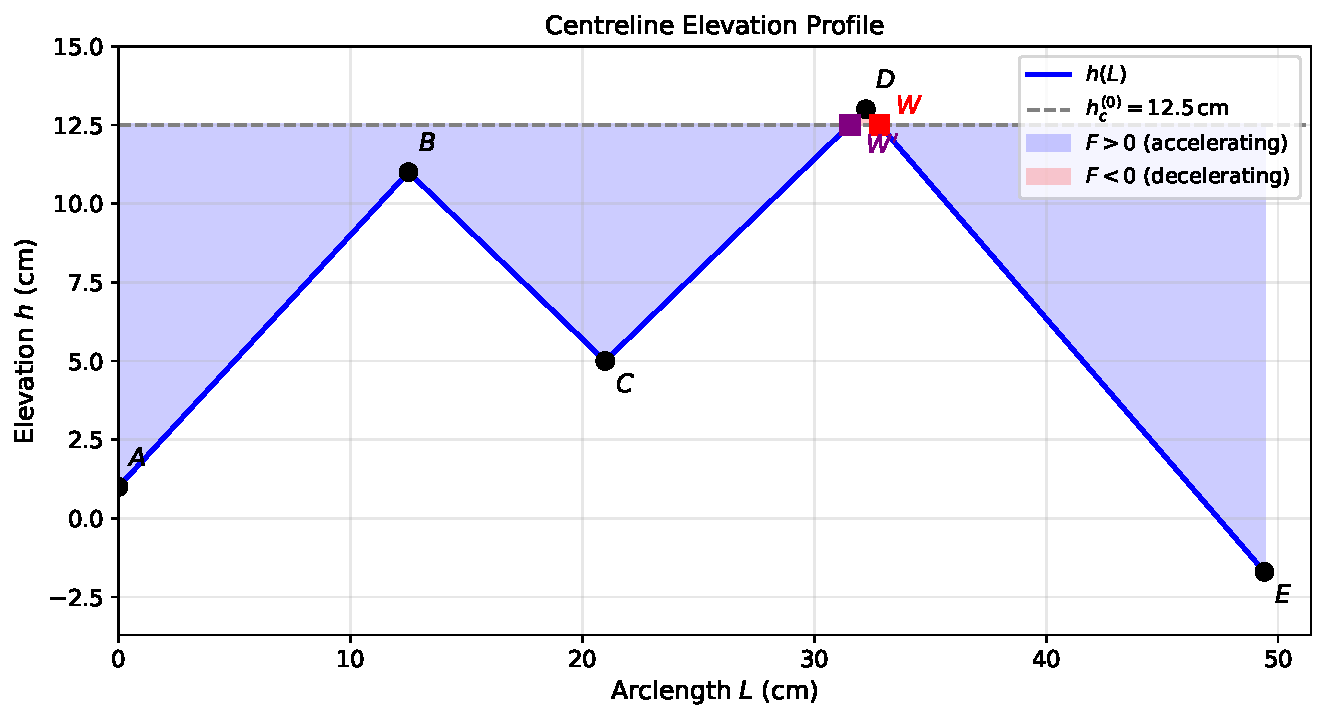
\includegraphics[width=0.9\textwidth]{figure2_centreline.pdf}
  \caption{Centreline elevation $h(L)$ versus arclength for the experimental geometry. The dashed line marks $h_c^{(0)} = 12.5$\,cm. After leaving $B$, the front crosses this level twice: once ascending (at $W'$ on $C \to D$) and once descending (at $W$ on $D \to E$). Blue shading: driving force positive. Red shading: driving force negative.}
  \label{fig:centreline}
\end{figure}

% ══════════════════════════════════════════════════════════════════════════════
%  SECTION 3: FRICTIONLESS MODEL
% ══════════════════════════════════════════════════════════════════════════════
\section{The Frictionless Model: Geometry Effects}
\label{sec:frictionless}

We begin with two idealising assumptions:
\begin{enumerate}[nosep,leftmargin=2em]
  \item \textbf{No friction}: Viscous losses neglected.
  \item \textbf{No drawdown}: Container level constant at $h_c^{(0)}$.
\end{enumerate}

These assumptions isolate the effect of geometry. Any geometry that fails here will certainly fail in reality.

\subsection{The driving force}

Consider the water in the pipe as a slug extending from the inlet to the front at position $L$. Forces on the slug:

\paragraph{Pressure at inlet.} The inlet at elevation $h_0$ is submerged to depth $h_c - h_0$. Hydrostatic pressure pushes the slug forward:
\[
  F_{\text{in}} = [p_{\text{atm}} + \rho g(h_c - h_0)] A.
\]

\paragraph{Pressure at front.} The front is open to atmospheric pressure in the empty pipe ahead:
\[
  F_{\text{front}} = p_{\text{atm}} A.
\]

\paragraph{Gravity along slug.} Integrating gravity along the slug from inlet (elevation $h_0$) to front (elevation $h(L)$):
\[
  F_{\text{gravity}} = -\rho g A [h(L) - h_0].
\]

The net driving force is:
\begin{align}
  F &= F_{\text{in}} - F_{\text{front}} + F_{\text{gravity}} \notag \\
    &= \rho g A (h_c - h_0) - \rho g A [h(L) - h_0] \notag \\
    &= \rho g A [h_c - h(L)].
  \label{eq:driving-force}
\end{align}

The inlet elevation cancels. The result depends only on the elevation difference between container surface and front:
\begin{equation}
  \boxed{F = \rho g A [h_c - h(L)]}
  \label{eq:driving-force-boxed}
\end{equation}

\paragraph{Sign of the driving force.}
\begin{itemize}[nosep,leftmargin=2em]
  \item $h(L) < h_c$: $F > 0$, slug accelerates, gains kinetic energy.
  \item $h(L) > h_c$: $F < 0$, slug decelerates, loses kinetic energy.
  \item $h(L) = h_c$: $F = 0$, slug coasts.
\end{itemize}

\paragraph{Acceleration.} Newton's second law with variable mass $m = \rho A L$:
\begin{equation}
  a = \frac{F}{\rho A L} = \frac{g[h_c - h(L)]}{L}.
  \label{eq:acceleration}
\end{equation}

Even when the force is large (e.g., at low point $C$ where $h_c - h(L) = 15$\,cm), the acceleration is suppressed by the growing slug length $L$.

\subsection{The energy integral}

Using $\ddot{L} = v \, dv/dL$ and the equation of motion $L \ddot{L} = g[h_c^{(0)} - h(L)]$:
\begin{equation}
  v \frac{dv}{dL} = \frac{g}{L}[h_c^{(0)} - h(L)].
  \label{eq:v-dv-dL}
\end{equation}

Integrating from $L = S_1$ (where $v = 0$) to general $L$:
\[
  \frac{1}{2}v^2 = g \int_{S_1}^{L} \frac{h_c^{(0)} - h(r)}{r} \, dr.
\]

Define the \emph{energy integral}:
\begin{equation}
  \boxed{I(L) = \int_{S_1}^{L} \frac{h_c^{(0)} - h(r)}{r} \, dr}
  \label{eq:energy-integral}
\end{equation}

Then:
\begin{equation}
  v(L) = \sqrt{2 g I(L)}, \qquad \text{provided } I(L) > 0.
  \label{eq:v-from-I}
\end{equation}

The integrand has two factors:
\begin{itemize}[nosep,leftmargin=2em]
  \item $h_c^{(0)} - h(r)$: the driving head at position $r$. Positive below waterline, negative above.
  \item $1/r$: the variable-mass weighting. Early contributions (short slug) are weighted more heavily.
\end{itemize}

The slug stalls when $I(L) = 0$.

\subsection{Priming criterion}

Priming succeeds if the slug reaches point $W$ with positive velocity:
\begin{equation}
  \boxed{I(S_W) > 0 \quad \Longleftrightarrow \quad \text{priming succeeds (frictionless)}}
  \label{eq:priming-criterion}
\end{equation}

Beyond $W$, the front is permanently below the waterline, so $I(L)$ only increases.

\subsection{Evaluation for piecewise-linear geometry}

On a segment where $h(r) = c + sr$, the contribution from interval $[a, b]$ is:
\begin{equation}
  \Phi(a, b; c, s) = (h_c^{(0)} - c) \ln\frac{b}{a} - s(b - a).
  \label{eq:Phi-def}
\end{equation}

To compute $I(L)$ for $L$ on segment $k$:
\begin{equation}
  I(L) = \sum_{j=2}^{k-1} \Phi(S_{j-1}, S_j; c_j, s_j) + \Phi(S_{k-1}, L; c_k, s_k).
  \label{eq:I-piecewise}
\end{equation}

\subsection{Evaluation for the experimental geometry}

Computing $I(S_W)$ for the experiment requires contributions from segments 2, 3, and part of 4.

\paragraph{Segment 2 ($B \to C$), interval $[12.50, 20.99]$\,cm:}
\[
  \Phi_2 = (12.5 - 19.84)\ln\frac{20.99}{12.50} - (-0.707)(8.49) = -3.80 + 6.00 = +2.20\,\text{cm}.
\]

\paragraph{Segment 3 ($C \to D$), interval $[20.99, 32.23]$\,cm:}
\[
  \Phi_3 = (12.5 - (-9.93))\ln\frac{32.23}{20.99} - (0.712)(11.24) = 9.62 - 8.00 = +1.62\,\text{cm}.
\]

\paragraph{Segment 4 ($D \to W$), interval $[32.23, 32.81]$\,cm:}
\[
  \Phi_4 = (12.5 - 40.57)\ln\frac{32.81}{32.23} - (-0.855)(0.58) = -0.50 + 0.50 = -0.005\,\text{cm}.
\]

\paragraph{Total:}
\begin{equation}
  I(S_W) = 2.20 + 1.62 - 0.005 = 3.82\,\text{cm} > 0.
  \label{eq:I-SW-value}
\end{equation}

The criterion is satisfied. Frictionless velocity at $W$:
\[
  v_W = \sqrt{2 \times 981 \times 3.82} = 86.5\,\text{cm/s} = 0.865\,\text{m/s}.
\]

\subsection{Design insights}

The energy integral reveals how geometry controls priming:

\begin{itemize}[nosep,leftmargin=2em]
  \item \textbf{Steep early drops are most effective.} The $\ln(b/a)$ weighting means early portions (small $r$) contribute more per unit length. The drop $B \to C$ occurs at $L \in [17, 31]$\,cm when the slug is short.

  \item \textbf{Part of the climb is ``free.''} Segment 3 contributes positively despite going uphill because part of it remains below the waterline.

  \item \textbf{The region above waterline costs energy.} The $\Phi_4 = -0.16$\,cm contribution is negative. Keep the crest low and the descent steep.

  \item \textbf{Screening without simulation.} The criterion $I(S_W) > 0$ is evaluated analytically. Geometries that fail can be rejected immediately.
\end{itemize}

% --- FIGURE 3: Driving force and acceleration ---
\begin{figure}[H]
  \centering
  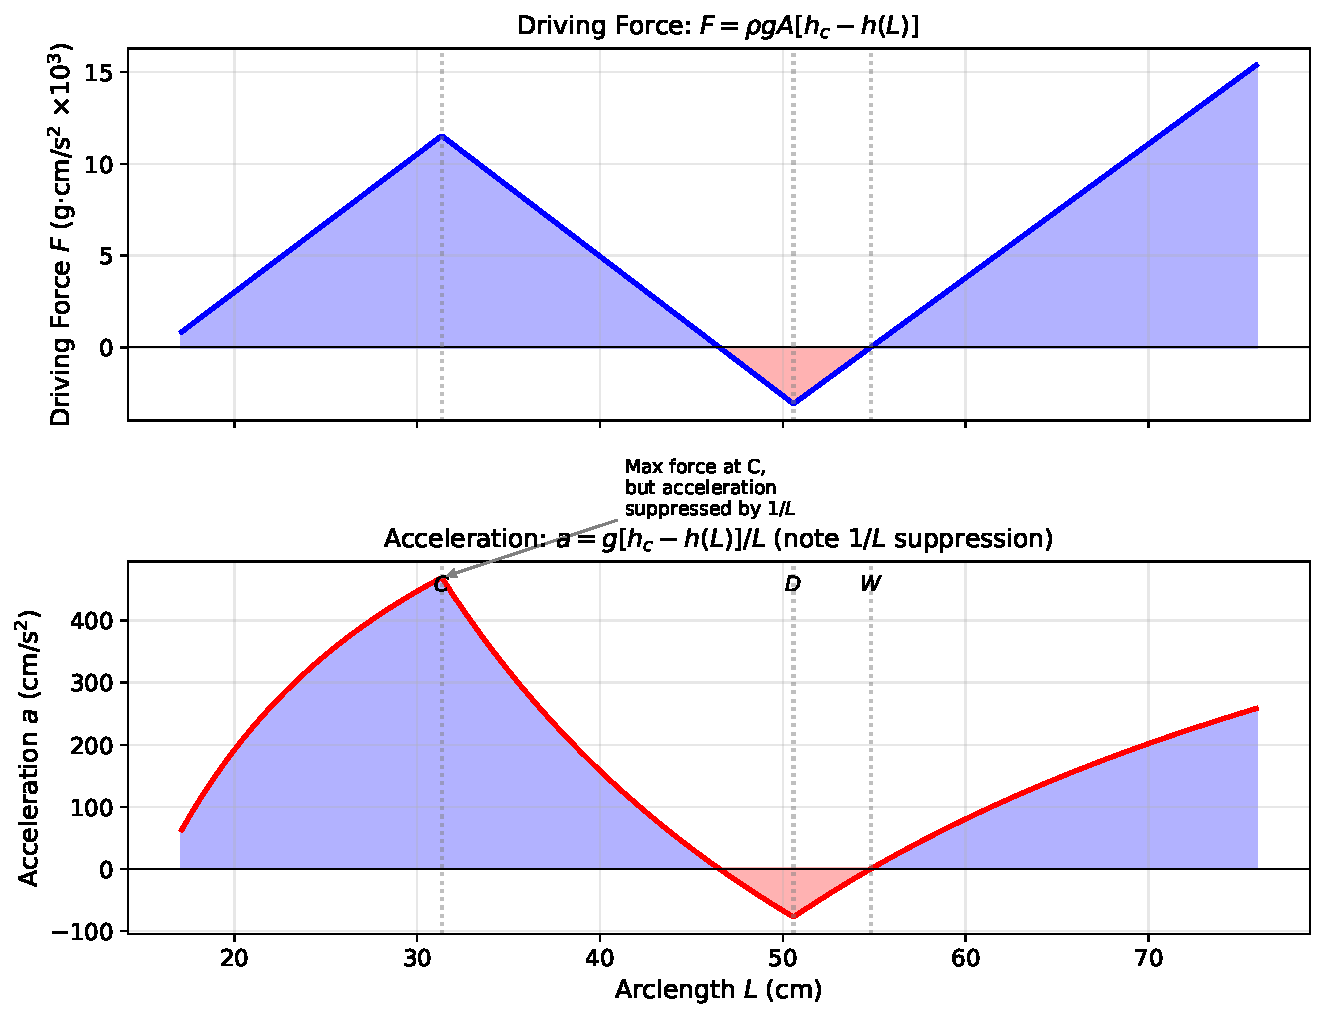
\includegraphics[width=0.9\textwidth]{figure3_force_acceleration.pdf}
  \caption{Top: Driving force $F(L) = \rho g A[h_c^{(0)} - h(L)]$ versus arclength. The force changes sign at waterline crossings. Bottom: Acceleration $a(L) = g[h_c^{(0)} - h(L)]/L$. Even at point $C$ where the force is maximum, the acceleration is moderated by the slug length $L$. The $1/L$ factor causes acceleration to decrease as the slug grows.}
  \label{fig:force-acceleration}
\end{figure}

% --- FIGURE 4: Energy integral I(L) ---
\begin{figure}[H]
  \centering
  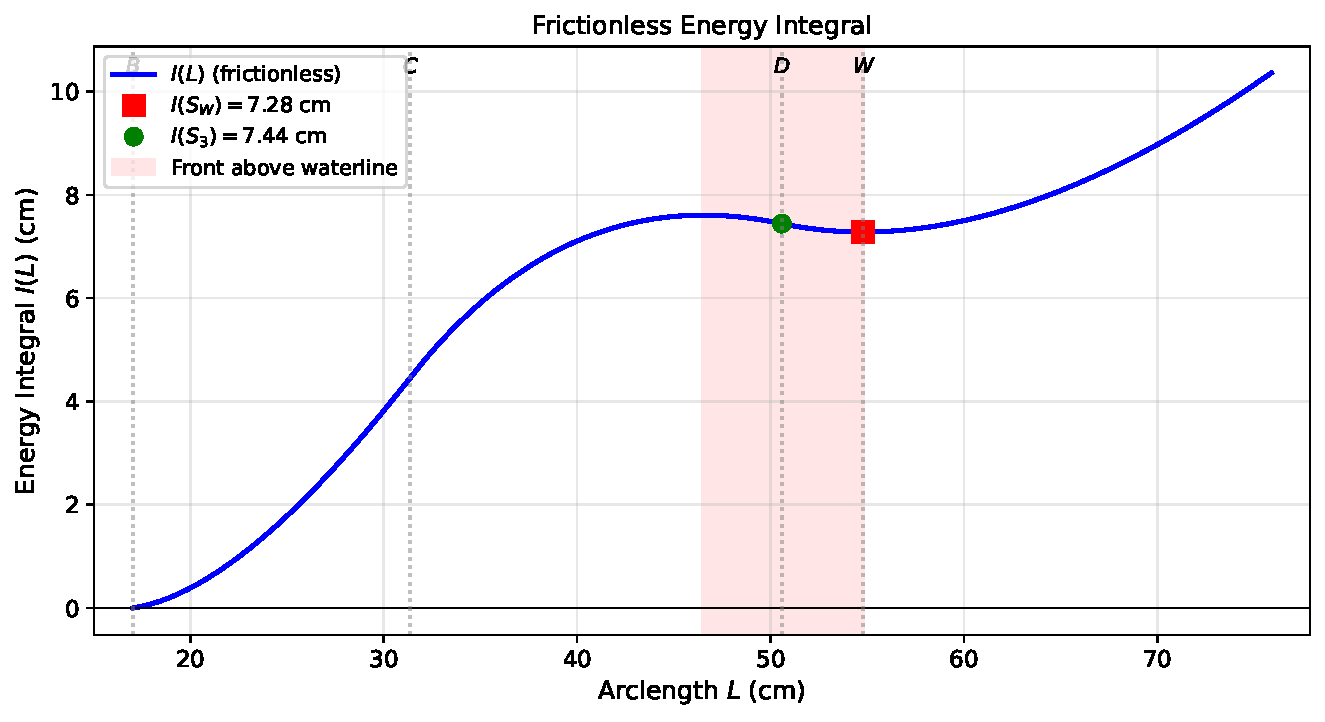
\includegraphics[width=0.9\textwidth]{figure4_energy_integral.pdf}
  \caption{Energy integral $I(L)$ versus arclength for the experimental geometry (frictionless, no drawdown). The integral rises during the drop $B \to C$, continues rising during the early climb (where $h < h_c^{(0)}$), then decreases slightly while the front is above the waterline (between $W'$ and $W$). At point $W$, $I(S_W) = 3.82$\,cm $> 0$: priming succeeds.}
  \label{fig:energy-integral}
\end{figure}

% ══════════════════════════════════════════════════════════════════════════════
%  SECTION 4: DRAWDOWN
% ══════════════════════════════════════════════════════════════════════════════
\section{Adding Container Drawdown: System Size Effects}
\label{sec:drawdown}

As water enters the pipe, the container level drops. This \emph{drawdown} reduces the driving force.

\subsection{The drawdown relation}

Volume conservation: water entering the pipe equals water leaving the container.
\[
  A(L - S_1) = A_0[h_c^{(0)} - h_c(L)].
\]

Solving:
\begin{equation}
  \boxed{h_c(L) = h_c^{(0)} - \frac{A}{A_0}(L - S_1)}
  \label{eq:drawdown}
\end{equation}

The container level decreases linearly with slug position at rate $A/A_0$.

\subsection{Modified energy integral}

With drawdown, the driving head becomes $h_c(L) - h(L)$ instead of $h_c^{(0)} - h(L)$. The energy integral becomes:
\begin{equation}
  I_{\text{dd}}(L) = \int_{S_1}^{L} \frac{h_c^{(0)} - \frac{A}{A_0}(r - S_1) - h(r)}{r} \, dr.
  \label{eq:I-dd-def}
\end{equation}

This splits into:
\begin{equation}
  I_{\text{dd}}(L) = I(L) - \frac{A}{A_0} \int_{S_1}^{L} \frac{r - S_1}{r} \, dr.
  \label{eq:I-dd-split}
\end{equation}

The drawdown penalty integral evaluates to:
\begin{equation}
  \int_{S_1}^{L} \frac{r - S_1}{r} \, dr = (L - S_1) - S_1 \ln\frac{L}{S_1}.
  \label{eq:drawdown-penalty}
\end{equation}

\subsection{Evaluation for the experimental geometry}

For the experiment with $A/A_0 = 5.77\times 10^{-4}$, at $L = S_W = 32.81$\,cm:
\[
  (32.81 - 12.50) - 12.50 \ln\frac{32.81}{12.50} = 20.31 - 12.06 = 8.25\,\text{cm}.
\]

Drawdown penalty:
\[
  \frac{A}{A_0} \times 8.25 = (5.77\times 10^{-4}) \times 8.25 = 0.0048\,\text{cm}.
\]

Modified integral:
\begin{equation}
  I_{\text{dd}}(S_W) = 3.82 - 0.005 = 3.81\,\text{cm} > 0.
  \label{eq:I-dd-value}
\end{equation}

Drawdown reduces the margin by only $\sim 0.1\%$ for this large container.

\subsection{When drawdown matters}

The total drawdown when the front reaches the outlet:
\[
  \Delta h_c = \frac{A}{A_0}(S_4 - S_1) = (5.77\times 10^{-4}) \times 36.91 = 0.021\,\text{cm}.
\]

For a smaller container with $A_0 = 20\,\text{cm}^2$ (area ratio $A/A_0 \approx 0.0098$):
\[
  \Delta h_c \approx 0.0098 \times 36.91 = 0.36\,\text{cm}.
\]

This would reduce the initial driving head of $h_c^{(0)} - h_1 = 1.5$\,cm at node $B$, potentially causing failure in marginal geometries.

\paragraph{Key parameter: $A/A_0$.} When $A/A_0 \ll 0.01$, drawdown is negligible. When $A/A_0 \gtrsim 0.01$, drawdown must be included.

% --- FIGURE 5: Container level h_c(L) ---
\begin{figure}[H]
  \centering
  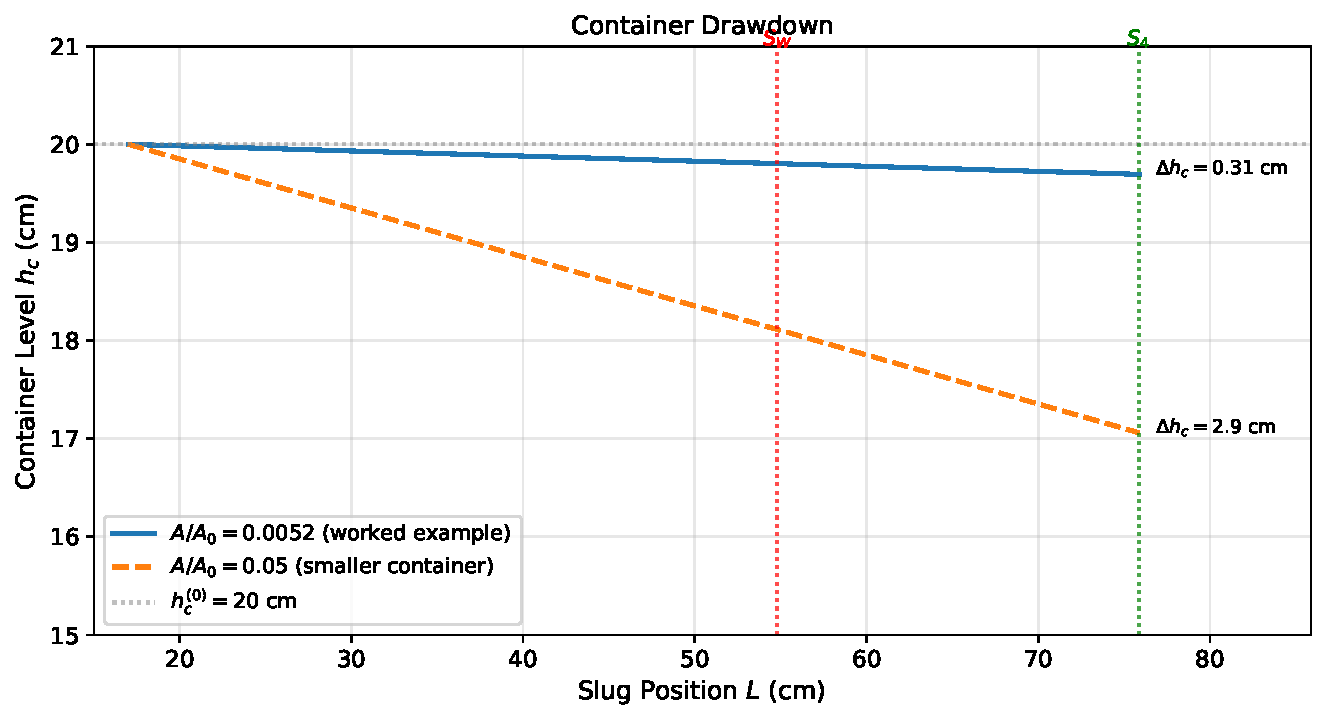
\includegraphics[width=0.9\textwidth]{figure5_drawdown.pdf}
  \caption{Container level $h_c(L)$ versus slug position for two area ratios. Solid line: $A/A_0 = 5.77\times 10^{-4}$ (experiment). Dashed line: $A/A_0 = 0.05$ (smaller container). Vertical dotted lines mark $S_W$ and $S_4$. For the experiment, drawdown is negligible ($\Delta h_c \approx 0.02$\,cm by the outlet).}
  \label{fig:drawdown}
\end{figure}

% ══════════════════════════════════════════════════════════════════════════════
%  SECTION 5: FRICTION
% ══════════════════════════════════════════════════════════════════════════════
\section{Adding Friction: Pipe Effects}
\label{sec:friction}

Viscous friction dissipates kinetic energy. We first develop a constant-friction model that preserves analytical tractability, then discuss velocity-dependent friction for the full dynamics.

\subsection{Friction head loss}

The Darcy-Weisbach equation gives the head loss over a pipe length $L$:
\begin{equation}
  h_f = f \frac{L}{D} \frac{v^2}{2g},
  \label{eq:darcy-weisbach}
\end{equation}
where $f$ is the Darcy friction factor.

Minor losses at bends add:
\begin{equation}
  h_{\text{minor}} = \sum K \frac{v^2}{2g}.
  \label{eq:minor-loss}
\end{equation}

Total head loss:
\begin{equation}
  h_{\text{loss}} = \left(f\frac{L}{D} + \sum K\right) \frac{v^2}{2g}.
  \label{eq:total-loss}
\end{equation}

\subsection{The constant-friction approximation}

The friction factor $f$ depends on Reynolds number $\text{Re} = vD/\nu$, which varies during filling. However, treating $f$ as constant enables analytical solution.

This approximation is exact in the fully rough regime where $f$ depends only on $\varepsilon/D$:
\begin{equation}
  \frac{1}{\sqrt{f}} = -2\log\left(\frac{\varepsilon/D}{3.7}\right).
  \label{eq:fully-rough}
\end{equation}

More generally, taking a representative value $f_0$ from the expected Reynolds number range introduces errors comparable to other model uncertainties. For the worked example, we use $f_0 \approx 0.078$, chosen from the filling-phase Reynolds number range after fitting $\sum K$ to the experimental $v(L)$ curve.

\subsection{Friction-corrected energy integral}

With constant friction and no drawdown, the equation of motion becomes:
\[
  v \frac{dv}{dL} + \left(\frac{f_0}{D} + \frac{\sum K}{L}\right) \frac{v^2}{2} = \frac{g}{L}[h_c^{(0)} - h(L)].
\]

Substituting $u = v^2/2$ gives a linear first-order ODE:
\begin{equation}
  \frac{du}{dL} + \left(\frac{f_0}{D} + \frac{\sum K}{L}\right) u = \frac{g}{L}[h_c^{(0)} - h(L)].
  \label{eq:u-ODE}
\end{equation}

The integrating factor is:
\begin{equation}
  \mu(L) = \left(\frac{L}{S_1}\right)^{\sum K} \exp\left(\frac{f_0(L - S_1)}{D}\right).
  \label{eq:integrating-factor}
\end{equation}

With $u(S_1) = 0$, the solution defines the \emph{friction-corrected energy integral}:
\begin{equation}
  \boxed{I_f(L) = \frac{1}{\mu(L)} \int_{S_1}^{L} \mu(r) \frac{h_c^{(0)} - h(r)}{r} \, dr}
  \label{eq:I-f-def}
\end{equation}
with $v(L) = \sqrt{2gI_f(L)}$.

\subsection{Physical interpretation}

In the frictionless integral, each position $r$ contributes with weight $1/r$. With friction, the effective weight becomes:
\[
  \frac{\mu(r)}{\mu(L)} \cdot \frac{1}{r} = \frac{1}{r}\left(\frac{r}{L}\right)^{\sum K} \exp\left(-\frac{f_0(L-r)}{D}\right).
\]

The exponential factor \emph{discounts} contributions from earlier positions: energy stored early has more distance to travel and suffers more dissipation. The prefactor $1/\mu(L)$ reflects cumulative dissipation over the entire path.

Since $\mu(r)/\mu(L) < 1$ for $r < L$, we have $I_f(L) < I(L)$ always.

\subsection{Evaluation for the experimental geometry}

The effective minor loss coefficient $\sum K = 14.4$ and relative roughness $\varepsilon/D$ were obtained by fitting the full ODE model (with velocity-dependent Churchill friction) to the measured velocity profile $v(L)$; the constant-friction approximation $f_0 \approx 0.078$ is the median friction factor from that calibrated solution. With $D = 0.5$\,cm, at $L = S_W = 32.81$\,cm:
\[
  \mu(S_W) = \left(\frac{32.81}{12.50}\right)^{14.4} \exp\left(\frac{0.078 \times 20.31}{0.5}\right) \approx (2.62)^{14.4} \times e^{3.16} \approx 2.5\times 10^{7}.
\]

Numerical evaluation gives:
\begin{equation}
  I_f(S_W) \approx 0.020\,\text{cm} > 0.
  \label{eq:I-f-value}
\end{equation}

Comparing to $I(S_W) = 3.82$\,cm, the constant-friction model reduces the available energy by $\sim 99.5\%$. The velocity at $W$:
\[
  v_W = \sqrt{2 \times 981 \times 0.020} \approx 6.3\,\text{cm/s} \approx 0.063\,\text{m/s}.
\]

The priming criterion is only marginally satisfied in the conservative constant-friction model. This reflects the experimental reality for a small-diameter siphon: effective minor losses (bends, entrance/exit, and unmodelled dissipation) can dominate the energy budget, leaving a small margin near the threshold.

\subsection{When friction matters}

The key parameters are $\varepsilon/D$ (relative roughness) and $\sum K$ (bend losses).

For the worked example, the measured peak filling velocity is $v \approx 0.36$\,m/s. With $D = 5$\,mm and $\nu = 10^{-6}\,\text{m}^2/\text{s}$:
\[
  \text{Re} \approx \frac{0.36 \times 0.005}{10^{-6}} \approx 1800,
\]
so the flow is mostly laminar and $f \approx 64/\text{Re} \approx 0.036$; roughness has little influence in this regime.

Distributed friction head loss over the full pipe ($L_{\max} = 0.494$\,m):
\[
  h_f \approx 0.036 \times \frac{0.494}{0.005} \times \frac{0.36^2}{2 \times 9.81} \approx 0.023\,\text{m} \approx 2.3\,\text{cm}.
\]

Minor losses (effective fitted $\sum K \approx 14.4$):
\[
  h_{\text{minor}} \approx 14.4 \times \frac{0.36^2}{2 \times 9.81} \approx 0.095\,\text{m} \approx 9.5\,\text{cm}.
\]

Thus, even at modest Reynolds numbers, minor losses can dominate the energy budget for small-diameter siphons. This motivates treating $\sum K$ as an effective parameter when bend details and entrance/exit effects are not measured.

% --- FIGURE 6: Friction factor f(Re) ---
\begin{figure}[H]
  \centering
  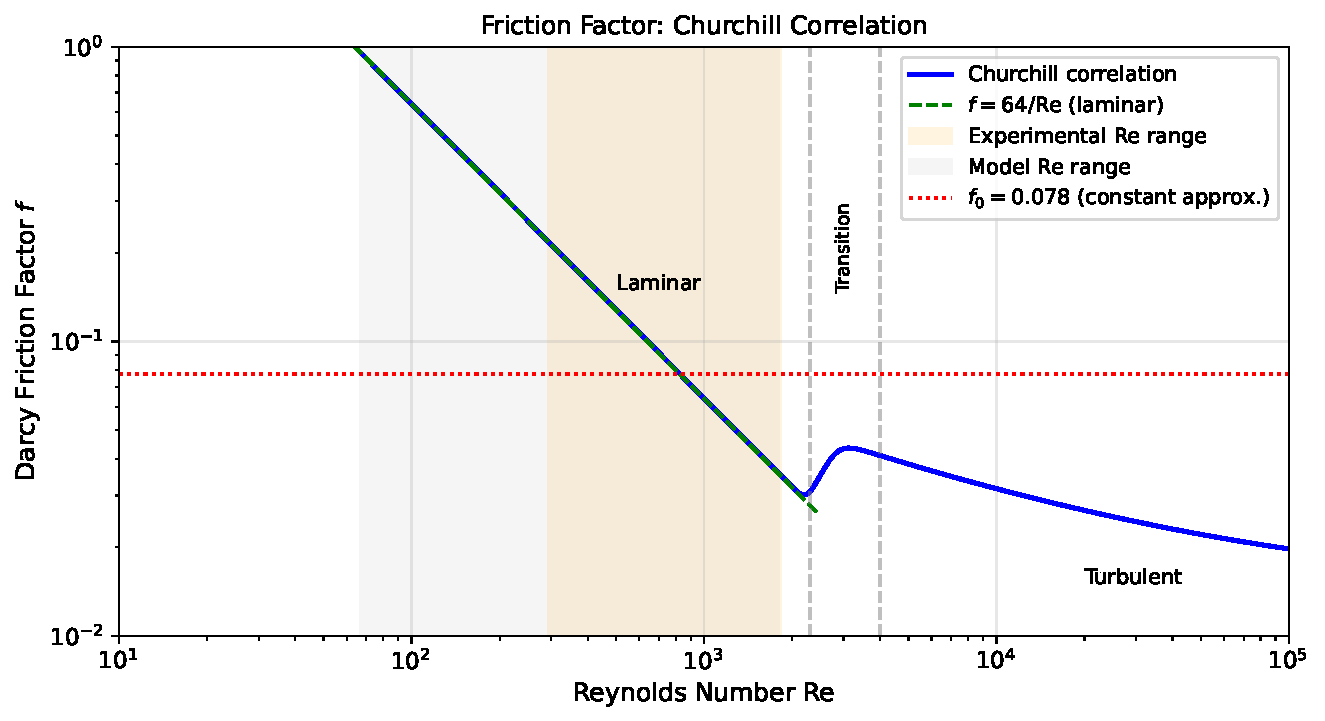
\includegraphics[width=0.9\textwidth]{figure6_friction.pdf}
  \caption{Friction factor $f$ versus Reynolds number from the Churchill correlation. Three regimes are visible: laminar ($f = 64/\text{Re}$), transitional, and turbulent. The shaded bands show the experimental and model Reynolds-number ranges during filling (both mostly below $\text{Re} \approx 2000$). The horizontal dashed line marks $f_0 \approx 0.078$, the constant-friction approximation.}
  \label{fig:friction}
\end{figure}

% ══════════════════════════════════════════════════════════════════════════════
%  SECTION 6: COMPARING THE THREE MODELS
% ══════════════════════════════════════════════════════════════════════════════
\section{Comparing the Three Models}
\label{sec:comparison}

We now have three energy integrals forming a hierarchy:
\begin{equation}
  I(L) \geq I_{\text{dd}}(L) \geq I_f(L).
  \label{eq:hierarchy}
\end{equation}

\subsection{Summary of values at $S_W$}

\begin{center}
\renewcommand{\arraystretch}{1.3}
\begin{tabular}{lccc}
\toprule
Model & Integral at $S_W$ & Velocity at $W$ & Key parameter \\
\midrule
Frictionless & $I = 3.82$\,cm & 0.865\,m/s & Geometry \\
With drawdown & $I_{\text{dd}} = 3.81$\,cm & 0.86\,m/s & $A/A_0 = 5.77\times 10^{-4}$ \\
With friction & $I_f \approx 0.020$\,cm & 0.063\,m/s & $\varepsilon/D$, $\sum K$ \\
\bottomrule
\end{tabular}
\end{center}

\subsection{Physical interpretation}

\paragraph{Frictionless integral $I(L)$:} The upper bound. Represents the maximum kinetic energy achievable from geometry alone. If $I(S_W) \leq 0$, no amount of friction reduction can save the design.

\paragraph{Drawdown-corrected integral $I_{\text{dd}}(L)$:} Accounts for the falling container level. The reduction $I - I_{\text{dd}}$ grows with $A/A_0$ and with slug length. For the worked example with a large container, drawdown reduces the margin by only $\sim 0.1\%$.

\paragraph{Friction-corrected integral $I_f(L)$:} Accounts for energy dissipation. For the worked example with an effective $\sum K \approx 14.4$, the constant-friction integral reduces the available energy by $\sim 99.5\%$. This substantial reduction arises from the $(L/S_1)^{\sum K}$ factor in the integrating factor together with the exponential discounting, both of which strongly penalise energy stored early along the path. The constant-friction model is conservative: it provides a lower bound that, while pessimistic, guarantees priming if $I_f(S_W) > 0$.

\subsection{Implications for geometry screening}

A geometry with $I(S_W) = 3$\,cm passes the frictionless test but may have $I_f(S_W) < 0$ and fail with friction. For the worked example with effective $\sum K \approx 14.4$, the constant-friction model predicts $I_f(S_W) \approx 0.020$\,cm---a small but positive margin. This sensitivity to minor losses suggests:
\begin{itemize}[nosep,leftmargin=2em]
  \item \textbf{Bend geometry matters more than pipe roughness.} The $\sum K$ term dominates.
  \item \textbf{Smoother bends dramatically improve margins.} Decreasing $\sum K$ significantly increases $I_f(S_W)$ and hence the priming margin.
  \item \textbf{The constant-friction model is conservative.} The full ODE with velocity-dependent friction typically predicts better performance.
\end{itemize}

% --- FIGURE 7: Comparison of three integrals ---
\begin{figure}[H]
  \centering
  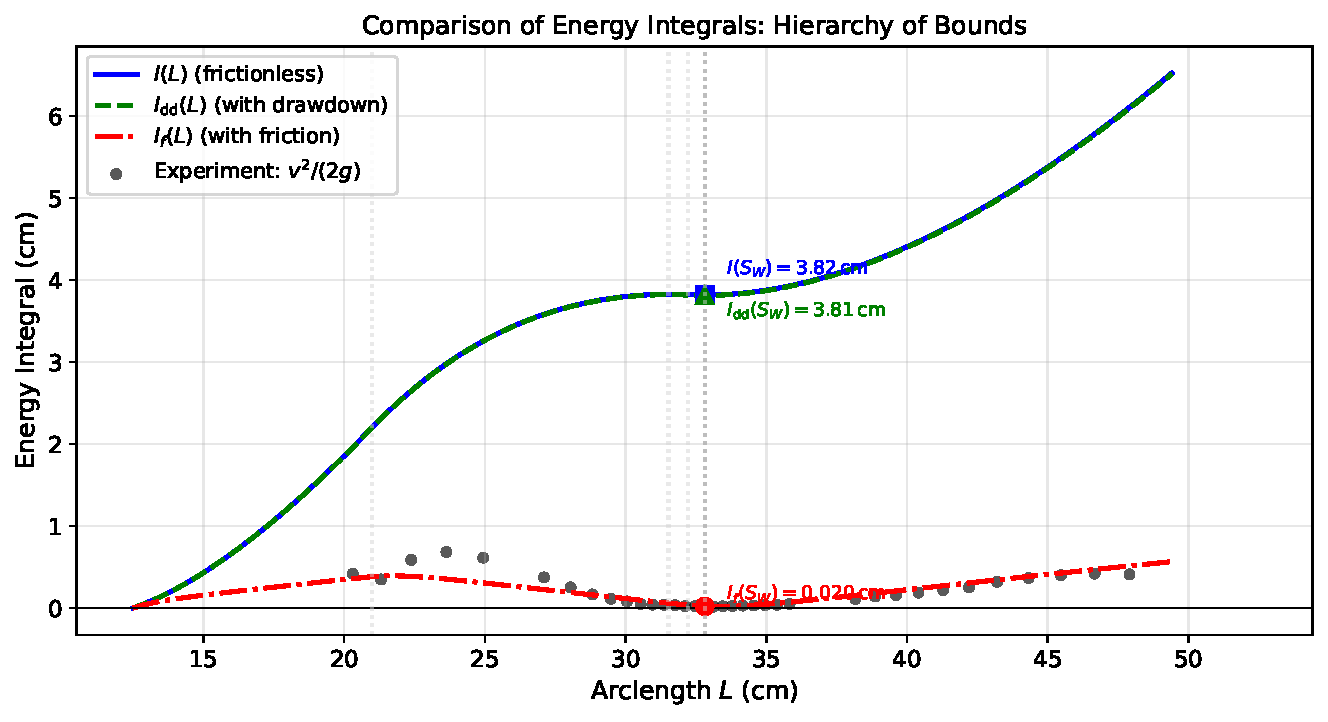
\includegraphics[width=0.9\textwidth]{figure7_comparison.pdf}
  \caption{Comparison of energy integrals $I(L)$, $I_{\text{dd}}(L)$, and $I_f(L)$ versus arclength for the worked example. The frictionless integral (solid) provides the upper bound. Drawdown (dashed) reduces it slightly. Friction (dash-dot) causes substantial reduction, especially as $L$ increases. Black points show the experimental kinetic head $v^2/(2g)$ plotted against biased $L$.}
  \label{fig:comparison}
\end{figure}

% ══════════════════════════════════════════════════════════════════════════════
%  SECTION 7: FULL DYNAMICS
% ══════════════════════════════════════════════════════════════════════════════
\section{The Full Dynamics}
\label{sec:dynamics}

The analytical integrals provide bounds and insight, but accurate predictions require velocity-dependent friction. This section develops the full equations and treats both filling and draining.

\subsection{Velocity-dependent friction: the Churchill correlation}

The friction factor depends on Reynolds number and relative roughness. The Churchill correlation provides a single formula valid across all flow regimes:
\begin{equation}
  f = 8\left[\left(\frac{8}{\text{Re}}\right)^{12} + \frac{1}{(A_C + B_C)^{3/2}}\right]^{1/12},
  \label{eq:churchill}
\end{equation}
where
\begin{align}
  A_C &= \left[2.457 \ln\left(\frac{1}{(7/\text{Re})^{0.9} + 0.27(\varepsilon/D)}\right)\right]^{16}, \\
  B_C &= \left(\frac{37530}{\text{Re}}\right)^{16}.
\end{align}

Key properties:
\begin{itemize}[nosep,leftmargin=2em]
  \item As $\text{Re} \to 0$: recovers $f = 64/\text{Re}$ (laminar).
  \item As $\text{Re} \to \infty$: recovers Colebrook-White (turbulent).
  \item Smooth interpolation through transition.
\end{itemize}

See \cref{app:friction} for details.

\subsection{Filling phase: equation of motion}

Including friction and drawdown:
\begin{equation}
  \boxed{\ddot{L} = \frac{g}{L}\left[h_c^{(0)} - \frac{A}{A_0}(L - S_1) - h(L)\right] - \left(\frac{f}{D} + \frac{\sum K}{L}\right)\frac{\dot{L}^2}{2}}
  \label{eq:filling-ODE}
\end{equation}

This is nonlinear due to:
\begin{itemize}[nosep,leftmargin=2em]
  \item Variable mass ($1/L$ factor)
  \item Piecewise-linear $h(L)$
  \item Velocity-dependent $f(\text{Re})$
  \item Quadratic friction ($\dot{L}^2$)
\end{itemize}

No closed-form solution exists.

\subsection{First-order system for numerical integration}

Define $v = \dot{L}$:
\begin{align}
  \frac{dL}{dt} &= v, \label{eq:system-L} \\
  \frac{dv}{dt} &= \frac{g}{L}\left[h_c^{(0)} - \frac{A}{A_0}(L - S_1) - h(L)\right] - \left(\frac{f}{D} + \frac{\sum K}{L}\right)\frac{v^2}{2}. \label{eq:system-v}
\end{align}

Initial conditions: $L(0) = S_1$, $v(0) = 0$.

At each integration step, compute $\text{Re} = vD/\nu$ and evaluate $f$ from \eqref{eq:churchill}.

\subsection{Comparison to experiment and analytical bounds}

Numerical integration for the experimental geometry yields:
\begin{itemize}[nosep,leftmargin=2em]
  \item Velocity at crest $D$: $\approx 0.08$\,m/s (vs.\ 0.87\,m/s frictionless)
  \item Velocity at $W$: $\approx 0.05$--$0.07$\,m/s (vs.\ 0.87\,m/s frictionless)
  \item Filling time to outlet: $\approx 2.2$\,s (experiment: $\sim 1.8$\,s of tracked filling)
\end{itemize}

The analytical bounds bracket reality:
\begin{itemize}[nosep,leftmargin=2em]
  \item Frictionless model overestimates velocity by $\sim 50$--$100\%$.
  \item Constant-friction model ($I_f$) is conservative. It provides a guaranteed lower bound but tends to underestimate actual performance, especially when minor losses are large.
  \item The full ODE captures velocity-dependent friction, giving intermediate results.
\end{itemize}

\subsection{Draining phase}
\label{sec:draining}

Once the front reaches the outlet ($L = L_{\max}$), the pipe is full and the system enters draining. The dynamics change because slug length is now constant.

\subsubsection{Full-pipe equation of motion}

With the pipe full at length $L_{\max}$:
\begin{equation}
  \dot{v} = \frac{g}{L_{\max}}[h_c(t) - h_4] - \frac{1}{L_{\max}}\left(f\frac{L_{\max}}{D} + \sum K\right)\frac{v^2}{2}.
  \label{eq:draining-v}
\end{equation}

\subsubsection{Container level evolution}

Volume flow rate $Q = Av$ removes water from the container:
\begin{equation}
  \frac{dh_c}{dt} = -\frac{A}{A_0}v.
  \label{eq:draining-hc}
\end{equation}

Equations \eqref{eq:draining-v} and \eqref{eq:draining-hc} form a coupled system for $(v, h_c)$ during draining.

\subsubsection{Quasi-steady approximation}

For large containers ($A/A_0 \ll 1$), the flow is approximately steady at each instant. Setting $\dot{v} = 0$:
\begin{equation}
  v_{\text{qs}} = \sqrt{\frac{2g(h_c - h_4)}{f\frac{L_{\max}}{D} + \sum K}}.
  \label{eq:quasi-steady}
\end{equation}

As the container drains, $h_c$ decreases and so does $v_{\text{qs}}$.

\subsubsection{Draining time estimate}

Substituting \eqref{eq:quasi-steady} into \eqref{eq:draining-hc} and integrating:
\begin{equation}
  t_{\text{drain}} = \frac{2A_0}{A}\sqrt{\frac{f\frac{L_{\max}}{D} + \sum K}{2g}}\sqrt{\Delta h_0},
  \label{eq:drain-time}
\end{equation}
where $\Delta h_0 = h_c^{(0)} - h_4$ is the initial siphon head.

For the worked example with $\Delta h_0 = h_c^{(0)} - h_4 = 12.5 - (-1.7) = 14.2$\,cm:
\[
  t_{\text{drain}} \approx \frac{2 \times 340}{0.196}\sqrt{\frac{0.078 \times (49.4/0.5) + 14.4}{2 \times 981}}\sqrt{14.2} \approx 1.4\times 10^{3}\,\text{s} \approx 23\,\text{min}.
\]

However, the experimentally observed drainage time was approximately 12 minutes---roughly half the quasi-steady prediction. This discrepancy suggests that the quasi-steady approximation, which assumes the friction factor remains constant at its fully-developed value throughout draining, overestimates the effective resistance. Possible explanations include: (i) the effective minor loss coefficient $\sum K$ fitted to filling-phase data may not apply unchanged during steady draining; (ii) air entrainment or intermittent flow near the end of draining may accelerate the process; (iii) the quasi-steady model neglects inertial effects during the initial acceleration to steady flow. For precise drainage-time predictions, the full coupled ODE system \eqref{eq:draining-v}--\eqref{eq:draining-hc} should be integrated numerically.

Draining is much slower than filling because friction limits the steady-state velocity.

\subsubsection{Draining terminates}

Draining continues until $h_c = h_4$ (siphon head zero) or until $h_c$ drops below the inlet ($h_c < h_0$), breaking the siphon by admitting air.

For the worked example with $h_0 = 1$\,cm and $h_4 = -1.7$\,cm, the siphon breaks when $h_c = h_0 = 1$\,cm. The container drains from 12.5\,cm to 1\,cm, removing:
\[
  \Delta V = A_0 \times 11.5\,\text{cm} = 340 \times 11.5 = 3910\,\text{cm}^3 \approx 3.9\,\text{L}.
\]

% --- FIGURE 8: Velocity v(L) comparison ---
\begin{figure}[H]
  \centering
  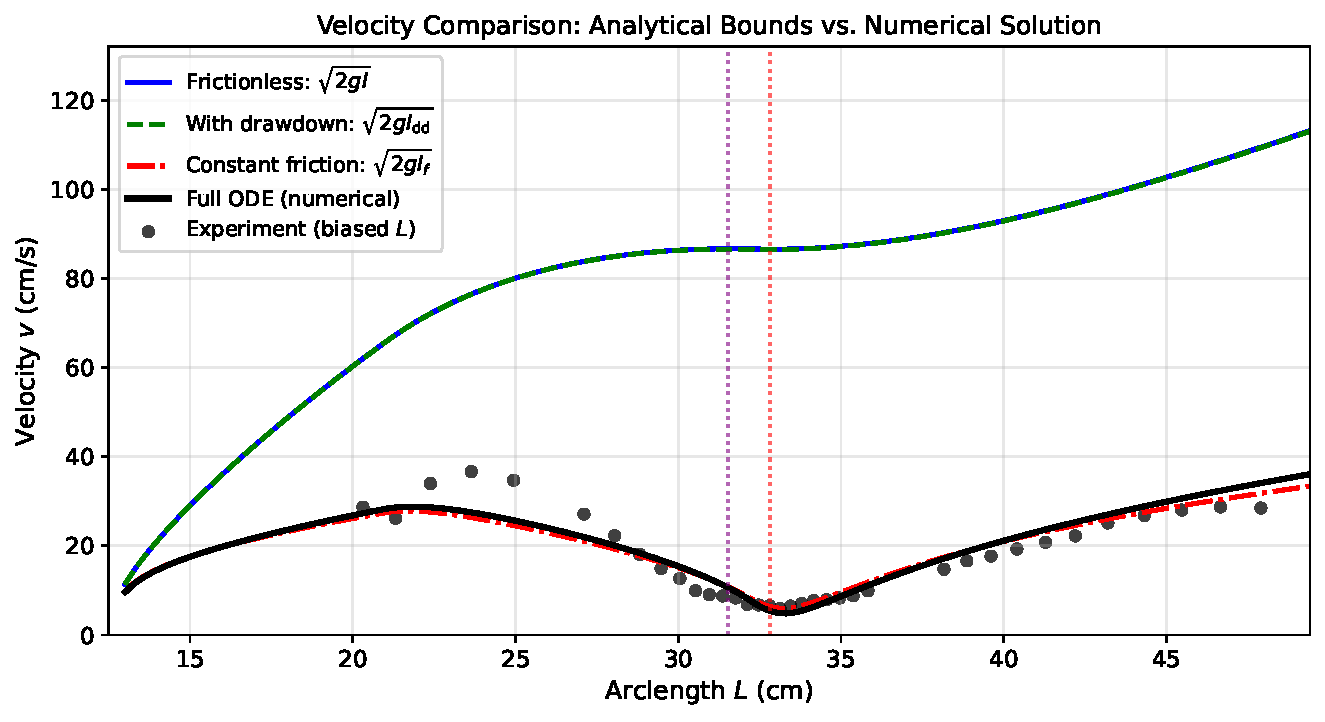
\includegraphics[width=0.9\textwidth]{figure8_velocity.pdf}
  \caption{Velocity $v(L)$ versus position during filling. Curves: frictionless $\sqrt{2gI}$, with drawdown $\sqrt{2gI_{\text{dd}}}$, constant friction $\sqrt{2gI_f}$, and full ODE numerical solution. Black points: experimental velocities plotted against the biased arclength $L$. The frictionless model overestimates velocity; the constant-friction model is conservative due to severe discounting of early-stored energy.}
  \label{fig:velocity}
\end{figure}

% --- FIGURE 9: Time evolution ---
\begin{figure}[H]
  \centering
  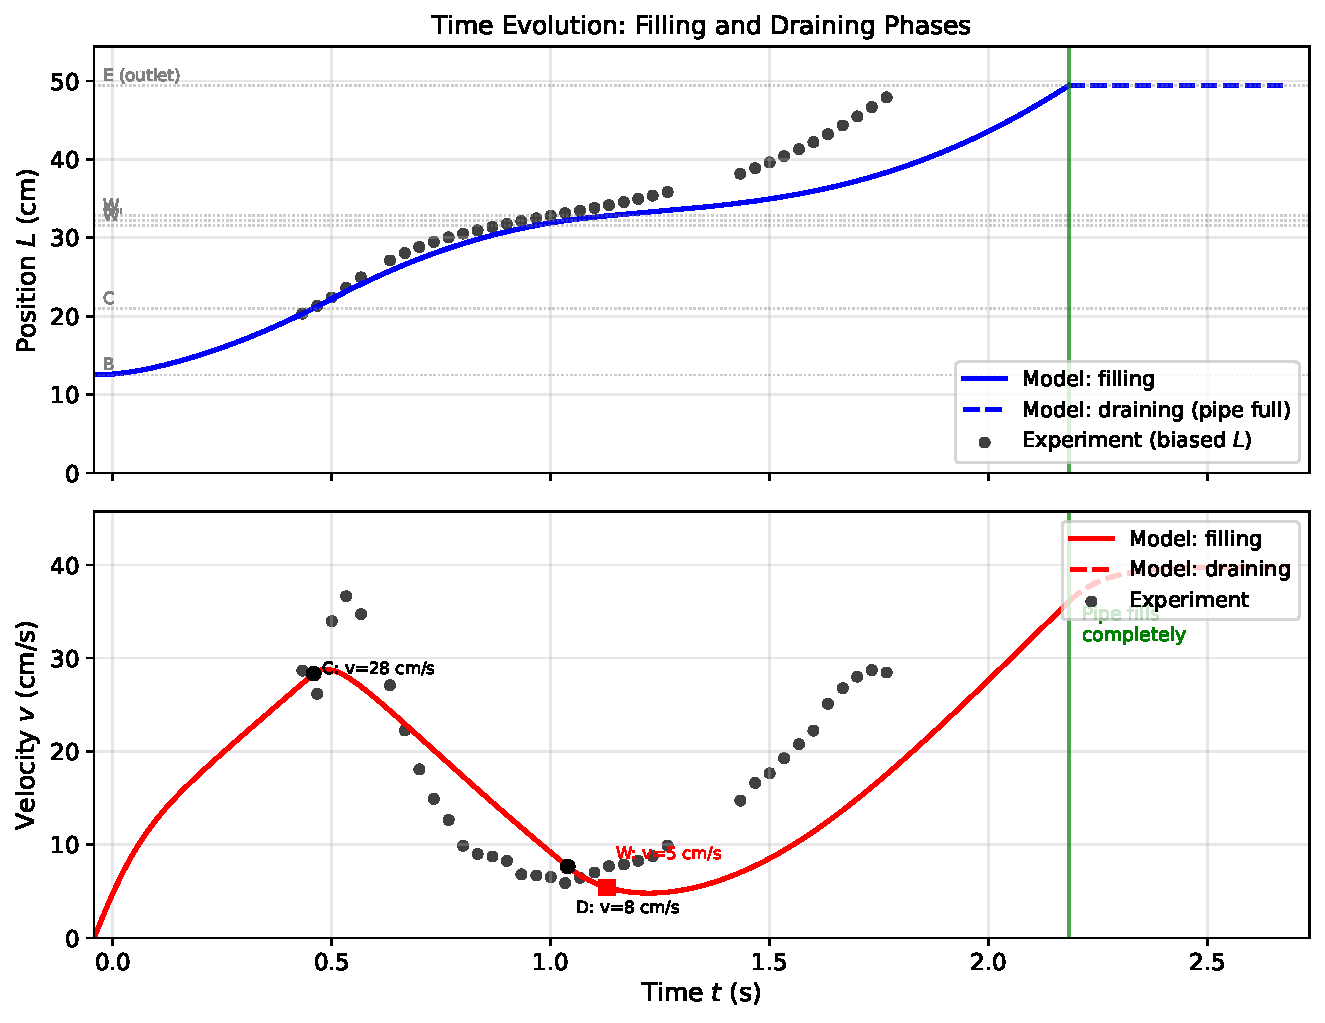
\includegraphics[width=0.9\textwidth]{figure9_time.pdf}
  \caption{Position $L(t)$ and velocity $v(t)$ versus time. Solid curves: numerical integration of the full ODE (time-shifted to align with the first experimental point). Black points: experimental $L_{\text{biased}}(t)$ and $v(t)$ from video tracking. Key points marked: $C$ (low point), $D$ (crest), $W$ (last waterline crossing), outlet.}
  \label{fig:time}
\end{figure}

% ══════════════════════════════════════════════════════════════════════════════
%  SECTION 8: NAVIER-STOKES DERIVATION
% ══════════════════════════════════════════════════════════════════════════════
\section{Foundations: Derivation from Navier-Stokes}
\label{sec:navier-stokes}

The preceding sections built the model from physical reasoning. This section derives it systematically from the Navier-Stokes equations, making every assumption explicit. The purpose is to clarify what the model captures and what it neglects, bridging to validity limits.

\subsection{The full equations}

For incompressible Newtonian fluid:
\begin{align}
  \nabla \cdot \mathbf{u} &= 0, \label{eq:NS-cont} \\
  \rho\left(\frac{\partial \mathbf{u}}{\partial t} + \mathbf{u} \cdot \nabla\mathbf{u}\right) &= -\nabla p + \mu\nabla^2\mathbf{u} + \rho\mathbf{g}. \label{eq:NS-mom}
\end{align}

These hold at every point. To obtain a one-dimensional model, we introduce assumptions.

\subsection{Step-by-step reduction}

\paragraph{Assumption 1: Axisymmetric flow in circular pipe.}
The pipe has circular cross-section with diameter $D$. Using cylindrical coordinates $(r, \theta, s)$ aligned with the pipe axis, the velocity is $\mathbf{u} = u_r\hat{r} + u_s\hat{s}$. For slender pipes ($D \ll L$), radial velocities are negligible: $u_r \ll u_s$.

\emph{What this neglects:} Non-circular cross-sections, three-dimensional effects at bends.

\paragraph{Assumption 2: Quasi-steady, fully-developed velocity profile.}
The instantaneous velocity profile matches the steady profile for the current mean velocity (parabolic for laminar, logarithmic for turbulent).

\emph{What this neglects:} Profile development time. Valid when flow changes slowly compared to viscous diffusion time $\tau_\nu = D^2/\nu$. For $D = 5$\,mm, $\tau_\nu \approx 25$\,s; filling occurs in $\sim 2$\,s, so this assumption is questionable during rapid acceleration.

\paragraph{Assumption 3: Cross-sectional averaging.}
Define mean velocity $\bar{u}(s,t)$ as the cross-sectional average of $u_s$. Integrating axial momentum over the cross-section:
\[
  \rho A \frac{\partial \bar{u}}{\partial t} + \rho A \bar{u}\frac{\partial \bar{u}}{\partial s} = -A\frac{\partial \bar{p}}{\partial s} + \tau_w \pi D + \rho g A \sin\theta,
\]
where $\tau_w = f\rho\bar{u}^2/8$ is wall shear stress.

\emph{What this neglects:} Radial pressure variations, momentum flux correction factors.

\paragraph{Assumption 4: Rigid slug with uniform velocity.}
The velocity is uniform along the slug: $\bar{u}(s,t) = v(t)$ for all $s$ in the wetted region. This eliminates $\partial\bar{u}/\partial s$.

\emph{What this neglects:} Compressibility, acoustic waves, spatial velocity variations.

\paragraph{Assumption 5: Hydrostatic boundary pressures.}
At the inlet: $p = p_{\text{atm}} + \rho g(h_c - h_0)$. At the front: $p = p_{\text{atm}}$.

\emph{What this neglects:} Dynamic pressure variations at boundaries, flow contraction at inlet.

\paragraph{Assumption 6: Incompressible fluid, rigid pipe walls.}
Fluid density $\rho$ is constant; pipe cross-section $A$ is constant.

\emph{What this neglects:} Compressibility effects, pipe wall deformation under pressure.

\subsection{Integration along the slug}

Integrating from inlet ($s = 0$) to front ($s = L$):

\paragraph{Inertia:}
\[
  \int_0^L \rho A \frac{\partial v}{\partial t} ds = \rho A L \dot{v}.
\]

\paragraph{Pressure:}
\[
  -\int_0^L A \frac{\partial \bar{p}}{\partial s} ds = A[p(0) - p(L)] = \rho g A(h_c - h_0).
\]

\paragraph{Gravity:}
\[
  \int_0^L \rho g A \sin\theta \, ds = \rho g A(h_0 - h(L)).
\]

\paragraph{Friction:}
\[
  \int_0^L \frac{f\rho v^2}{8}\pi D \, ds = \rho A f \frac{L}{D}\frac{v^2}{2}.
\]

Combining and dividing by $\rho A L$:
\[
  \dot{v} = \frac{g}{L}[h_c - h(L)] - \frac{f}{D}\frac{v^2}{2}.
\]

This recovers \eqref{eq:filling-ODE} without minor losses (which require separate treatment of localised pressure drops).

\subsection{Summary of assumptions}

\begin{center}
\renewcommand{\arraystretch}{1.3}
\begin{tabular}{clll}
\toprule
\# & Assumption & What it neglects & Failure mode \\
\midrule
1 & Axisymmetric, circular pipe & 3D effects at bends & Tight bends \\
2 & Quasi-steady velocity profile & Profile development & Rapid acceleration \\
3 & Cross-sectional averaging & Radial variations & Large $D/L$ \\
4 & Rigid slug, uniform velocity & Compressibility & High velocity \\
5 & Hydrostatic boundaries & Dynamic effects & Fast flows \\
6 & Incompressible, rigid walls & Compressibility & Very high pressure \\
\bottomrule
\end{tabular}
\end{center}

% ══════════════════════════════════════════════════════════════════════════════
%  SECTION 9: VALIDITY LIMITS
% ══════════════════════════════════════════════════════════════════════════════
\section{Validity Limits}
\label{sec:validity}

Every model has a domain of validity. Understanding where it breaks down is as important as knowing where it works. This section quantifies when each assumption fails.

\subsection{Overview}

The assumptions from \cref{sec:navier-stokes} break down when:
\begin{itemize}[nosep,leftmargin=2em]
  \item Pressure drops below vapour pressure $\to$ cavitation
  \item Surface tension dominates $\to$ capillarity effects
  \item Flow changes rapidly $\to$ unsteady friction
  \item Bends are tight $\to$ three-dimensional effects
\end{itemize}

Each limit is characterised by a dimensionless parameter with a critical threshold.

\subsection{Cavitation}

\subsubsection{Physical mechanism}

At the highest point (crest $D$), pressure is lowest. If it drops below the vapour pressure $p_v \approx 2.3$\,kPa, dissolved gases emerge, breaking the liquid column.

\subsubsection{Quantitative criterion}

Using Bernoulli along the slug to the crest:
\[
  p_D = p_{\text{atm}} + \rho g(h_c - h_3) - \frac{1}{2}\rho v^2 - \rho g h_f.
\]

Cavitation occurs when $p_D < p_v$. The maximum crest height is:
\begin{equation}
  h_3 - h_c < \frac{p_{\text{atm}} - p_v}{\rho g} - \frac{v^2}{2g} - h_f \approx 10\,\text{m} - \frac{v^2}{2g} - h_f.
  \label{eq:cavitation-criterion}
\end{equation}

For water, atmospheric pressure supports $\sim 10$\,m. Velocity head and friction losses reduce this margin.

\subsubsection{Worked example assessment}

At frictionless crest velocity $v = 1.21$\,m/s with $h_3 - h_c = 4$\,cm:
\[
  p_D \approx 101300 + 1000 \times 9.81 \times (-0.04) - \frac{1}{2} \times 1000 \times 1.21^2 \approx 100200\,\text{Pa}.
\]

This is well above $p_v = 2300$\,Pa. Cavitation margin: $(100200 - 2300)/(1000 \times 9.81) \approx 10$\,m. Cavitation is not a concern.

\subsection{Capillarity}

\subsubsection{Physical mechanism}

At small diameters, surface tension affects front dynamics. The meniscus curvature creates a capillary pressure:
\[
  \Delta p_{\text{cap}} = \frac{4\gamma\cos\theta_c}{D},
\]
where $\theta_c$ is the contact angle ($\theta_c \approx 0$ for water on clean glass/plastic).

\subsubsection{Quantitative criteria}

The Bond number compares gravity to surface tension:
\begin{equation}
  \text{Bo} = \frac{\rho g D^2}{\gamma}.
  \label{eq:bond}
\end{equation}

Capillarity is negligible when $\text{Bo} \gg 1$.

The capillary number compares viscous to capillary forces:
\begin{equation}
  \text{Ca} = \frac{\mu v}{\gamma}.
  \label{eq:capillary}
\end{equation}

Dynamic meniscus effects are negligible when $\text{Ca} \ll 1$.

\subsubsection{Worked example assessment}

For $D = 5$\,mm:
\[
  \text{Bo} = \frac{1000 \times 9.81 \times 0.005^2}{0.073} \approx 3.4.
\]

Capillary pressure: $\Delta p_{\text{cap}} = 4 \times 0.073/0.005 \approx 58$\,Pa, corresponding to head $\approx 0.6$\,cm. This is $\sim 40\%$ of the initial driving head of $h_c^{(0)} - h_1 = 1.5$\,cm---not negligible for this diameter.

At the measured peak filling speed $v \approx 0.36$\,m/s:
\[
  \text{Ca} = \frac{10^{-3} \times 0.36}{0.073} \approx 0.0049.
\]

Small $\text{Ca}$ indicates viscous-capillary coupling at the meniscus is possible, especially near the crest where velocities are small.

\paragraph{Recommendation:} For $D > 15$\,mm, capillarity is negligible. For $D < 5$\,mm, capillarity dominates. The worked example at $D = 5$\,mm lies near the capillary-influenced boundary.

\subsection{Entrance effects and unsteady friction}

\subsubsection{Physical mechanism}

The quasi-steady friction model assumes the velocity profile instantaneously adjusts. In reality, the profile develops over an entrance length $L_e$, and rapid acceleration produces transient shear stresses.

\subsubsection{Quantitative criteria}

Entrance length (turbulent):
\begin{equation}
  L_e \approx 10D \text{ to } 20D.
  \label{eq:entrance}
\end{equation}

Strouhal number characterises unsteady effects:
\begin{equation}
  \text{St} = \frac{D}{vT},
  \label{eq:strouhal}
\end{equation}
where $T$ is the characteristic time of velocity change. Unsteady effects are small when $\text{St} \ll 1$.

The Womersley number characterises oscillatory flows:
\begin{equation}
  \text{Wo} = D\sqrt{\frac{\omega}{\nu}},
  \label{eq:womersley}
\end{equation}
where $\omega$ is angular frequency. For filling, $\omega \sim 1/T$.

\subsubsection{Worked example assessment}

For the worked example, the flow is mostly laminar ($\text{Re} \lesssim 2000$). Laminar entrance length scales as $L_e/D \approx 0.05\,\text{Re}$, so at $\text{Re} \approx 1800$:
\[
  \frac{L_e}{D} \approx 90 \quad \Rightarrow \quad L_e \approx 90 \times 0.5\,\text{cm} \approx 45\,\text{cm}.
\]
Segments are 8--17\,cm, so the flow is likely developing over much of the pipe; this is a plausible source of deviation from quasi-steady friction assumptions.

For $v \approx 0.36$\,m/s changing over $T = 0.5$\,s:
\[
  \text{St} = \frac{0.005}{0.36 \times 0.5} \approx 0.028.
\]

Small Strouhal number suggests unsteady effects are modest, but they may matter during initial acceleration and near the crest where velocities are low.

\subsection{Three-dimensional effects at bends}

\subsubsection{Physical mechanism}

Flow through bends generates secondary flows (Dean vortices) that enhance mixing and dissipation. The minor loss coefficients $K$ empirically capture these effects.

\subsubsection{Quantitative criterion}

The Dean number characterises secondary flow intensity:
\begin{equation}
  \text{De} = \text{Re}\sqrt{\frac{D}{2R}},
  \label{eq:dean}
\end{equation}
where $R$ is the bend radius of curvature. Secondary flows are significant when $\text{De} > 100$.

\subsubsection{Worked example assessment}

For tight $180^\circ$ bends with $R \approx 2D$ and $\text{Re} \approx 1800$:
\[
  \text{De} \approx 1800 \times \sqrt{\frac{1}{4}} \approx 900.
\]

This Dean number indicates strong secondary flows. In practice, entrance/exit effects and bend losses can be absorbed into an effective $\sum K$ when detailed bend geometry is not characterised; in the worked example, fitting to the measured $v(L)$ yields $\sum K \approx 14.4$ (order $3$--$4$ per bend for four bends).

\subsection{Validity regime diagrams}

\Cref{fig:validity} presents the validity limits in three parameter spaces.

% --- FIGURE 10: Validity regime diagrams ---
\begin{figure}[H]
  \centering
  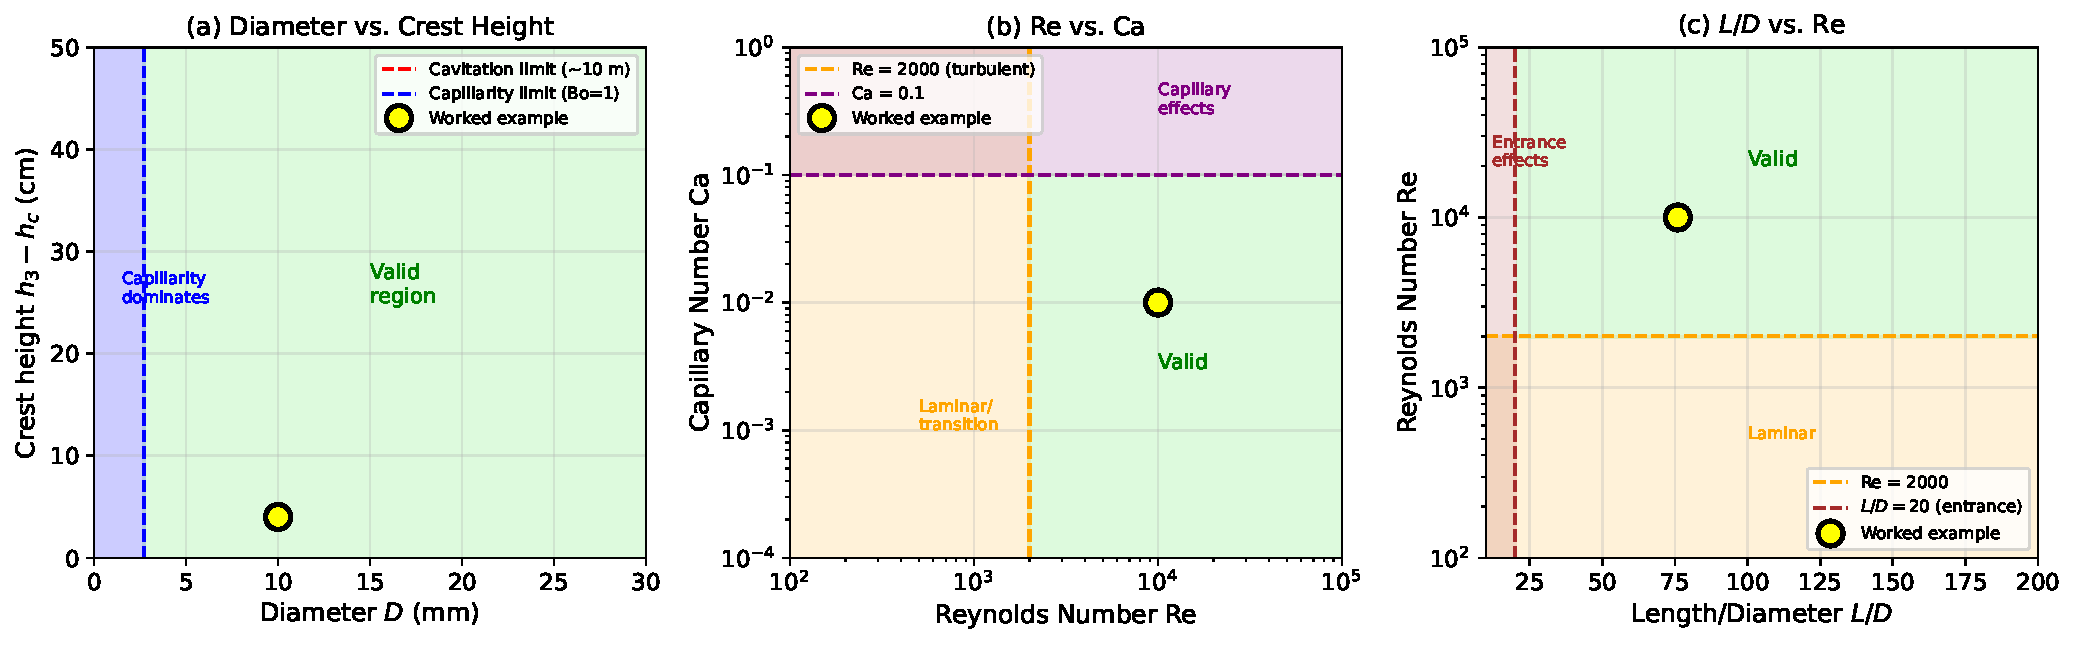
\includegraphics[width=0.95\textwidth]{figure10_validity.pdf}
  \caption{Validity regime diagrams. (a) Diameter $D$ versus crest height $h_3 - h_c$: cavitation limits tall crests; capillarity limits small diameters. (b) Reynolds number versus capillary number: highlights the laminar/transition boundary and the small-$\text{Ca}$ regime. (c) $L/D$ versus Reynolds number: high $L/D$ means friction-dominated flow; entrance-length and quasi-steady assumptions become questionable at low Re. The worked example (marked) lies close to the capillary/entrance-effect boundaries.}
  \label{fig:validity}
\end{figure}

\subsubsection{Diagram (a): $D$ versus $h_3 - h_c$}

Upper boundary: cavitation limit, $(h_3 - h_c) < 10\,\text{m} - v^2/2g$. Lower boundary for small $D$: capillarity dominates when $\text{Bo} < 1$, i.e., $D < \sqrt{\gamma/\rho g} \approx 2.7$\,mm.

\emph{Insight:} The worked example ($D = 5$\,mm, $h_3 - h_c = 0.5$\,cm) is far from cavitation but close to the capillary-influenced regime.

\subsubsection{Diagram (b): Re versus Ca}

Valid region: $\text{Ca} < 0.1$ (capillary effects on meniscus small) and sufficiently high Re for quasi-steady/fully-developed assumptions. The worked example operates at $\text{Re} \sim 10^3$, $\text{Ca} \sim 5\times 10^{-3}$: capillary number is small, but Re is near the laminar/transition boundary, so developing-flow effects may matter.

\emph{Insight:} Decreasing diameter pushes toward higher Re (for fixed velocity) but also higher capillary influence. There is an optimal diameter range.

\subsubsection{Diagram (c): $L/D$ versus Re}

For quasi-steady friction, each segment should exceed entrance length. Using the turbulent estimate $L_e \approx 10D$ to $20D$, the worked example has $L_i/D \approx 17$ to 34 and would be marginal. In the laminar regime, however, entrance lengths can be much longer ($L_e/D \sim 0.05\,\text{Re}$), so this is a key limitation.

\emph{Insight:} Shorter segments or smaller diameters push toward the entrance-effect-dominated regime where the friction model loses accuracy.

\subsubsection{Summary}

The worked example lies near the capillary and entrance-effect boundaries. This suggests that discrepancies between the simplest 1D model and experiment may be driven by meniscus physics and developing/unsteady friction, rather than by geometry alone.

% ══════════════════════════════════════════════════════════════════════════════
%  SECTION 10: CONCLUSION
% ══════════════════════════════════════════════════════════════════════════════
\section{Conclusion}
\label{sec:conclusion}

This paper developed a theoretical framework for investigating self-starting siphons through layered analysis.

The frictionless model isolates geometry as the controlling parameter. The energy integral $I(L)$ accumulates contributions to kinetic energy, weighted by $1/L$ to account for the growing slug mass. The priming criterion $I(S_W) > 0$ is computable in closed form for piecewise-linear geometries.

Adding drawdown introduces the area ratio $A/A_0$. The modified integral $I_{\text{dd}}(L)$ remains analytical. For large containers ($A/A_0 < 0.01$), drawdown is negligible.

Adding friction introduces $\varepsilon/D$ and the bend loss coefficients $K$. The constant-friction integral $I_f(L)$ reveals how dissipation discounts early-stored energy through an exponential factor. This intermediate model provides conservative velocity estimates.

Comparing the three integrals on a single graph visualises the energy cost of each effect. For the experimental geometry with effective $\sum K \approx 14.4$, the constant-friction model predicts that friction dominates, reducing energy by $\sim 99.5\%$; drawdown accounts for only $\sim 0.1\%$. Experimental velocity measurements confirm the hierarchy: the frictionless model overestimates, the constant-friction model is conservative, and the full ODE provides the closest match. This sensitivity to minor losses highlights the importance of bend geometry: larger $\sum K$ would reduce the available energy much more severely.

The full dynamics require numerical integration due to velocity-dependent friction, but the analytical integrals bracket the solution. The draining phase, which dominates the total siphoning time, is governed by a simpler ODE where the slug length is constant.

Derivation from Navier-Stokes makes every assumption explicit, bridging to validity limits. Cavitation, capillarity, entrance effects, and three-dimensional bend flows each have characteristic dimensionless parameters. Regime diagrams show where the model is reliable and where it may fail.

The framework enables systematic parameter investigation:
\begin{itemize}[nosep,leftmargin=2em]
  \item \textbf{Geometry} controls the frictionless energy budget---the fundamental determinant of priming.
  \item \textbf{Pipe properties} ($D$, $\varepsilon/D$, $K$) control friction losses.
  \item \textbf{System size} ($A/A_0$) controls drawdown.
  \item \textbf{Optimal designs minimise bend losses.} Once geometry ensures $I(S_W) > 0$, reducing minor loss coefficients (lowering $\sum K$ with smooth, gentle bends) is typically the most effective way to increase the priming margin and reduce filling time.
\end{itemize}

Changes that improve priming generally also speed filling: steeper drops, lower crests, larger diameters, smoother pipes. The exception is container size: larger containers ease priming but extend draining time.

The model provides analytical insight into how each parameter affects the siphoning process---the understanding that numerical simulation alone cannot offer.

% ══════════════════════════════════════════════════════════════════════════════
%  APPENDIX: FRICTION CORRELATIONS
% ══════════════════════════════════════════════════════════════════════════════
\appendix
\section{Friction Correlations}
\label{app:friction}

\subsection{The Churchill correlation}

The Churchill (1977) correlation provides a single formula for the Darcy friction factor valid across all flow regimes:
\begin{equation}
  f = 8\left[\left(\frac{8}{\text{Re}}\right)^{12} + \frac{1}{(A_C + B_C)^{3/2}}\right]^{1/12},
  \label{eq:churchill-full}
\end{equation}
where
\begin{align}
  A_C &= \left[2.457\ln\left(\frac{1}{(7/\text{Re})^{0.9} + 0.27(\varepsilon/D)}\right)\right]^{16}, \\
  B_C &= \left(\frac{37530}{\text{Re}}\right)^{16}.
\end{align}

\subsection{Limiting behaviour}

\paragraph{Laminar limit ($\text{Re} \to 0$):}
The first term $(8/\text{Re})^{12}$ dominates. Expanding:
\[
  f \to 8 \times \frac{8}{\text{Re}} = \frac{64}{\text{Re}},
\]
the exact Hagen-Poiseuille result.

\paragraph{Turbulent limit ($\text{Re} \to \infty$):}
The second term dominates. As $B_C \to 0$, $f \to 8/(A_C)^{1/8}$, which recovers the Colebrook-White equation:
\[
  \frac{1}{\sqrt{f}} = -2\log\left(\frac{\varepsilon/D}{3.7} + \frac{2.51}{\text{Re}\sqrt{f}}\right).
\]

\paragraph{Transition region:}
Both terms contribute, providing smooth interpolation. The resulting $f$ is continuous and differentiable.

\subsection{Comparison to Colebrook-White}

The Colebrook-White equation is implicit and requires iteration. Explicit approximations (Haaland, Swamee-Jain) introduce 1--2\% error. Churchill matches Colebrook-White in the turbulent regime to within 1\% while also covering laminar flow.

For siphon filling where Re spans from 0 to $\sim 10^4$, Churchill is the natural choice: it requires no regime-switching logic and handles the entire range consistently.

\subsection{Accuracy considerations}

Colebrook-White itself is an empirical fit to Nikuradse's 1930s experiments, with accuracy $\pm 5$--$10\%$. The uncertainty in friction factor is comparable to uncertainties in minor loss coefficients and the quasi-steady assumption. For parameter investigation, the Churchill correlation is more than adequate.

% --- FIGURE A1: Friction correlation comparison ---
\begin{figure}[H]
  \centering
  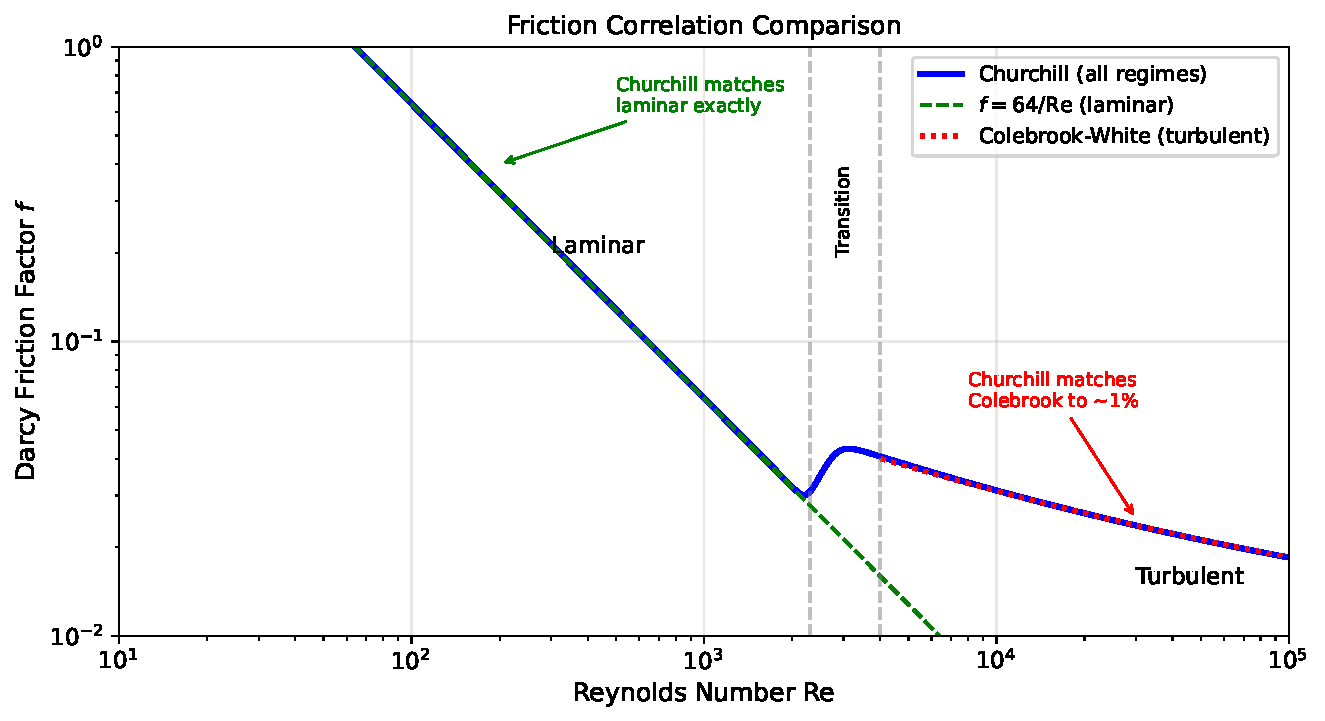
\includegraphics[width=0.9\textwidth]{figureA1_friction_comparison.pdf}
  \caption{Comparison of friction correlations. Solid: Churchill. Dashed: Colebrook-White (turbulent only). Dotted: $f = 64/\text{Re}$ (laminar). The Churchill correlation bridges all regimes smoothly. For $\text{Re} > 4000$, it matches Colebrook-White to within 1\%.}
  \label{fig:friction-comparison}
\end{figure}

\end{document}
